\documentclass[11pt]{article}
\usepackage[a4paper,margin=25mm]{geometry}
\usepackage{amsmath,amssymb,amsthm}
\usepackage{fontspec}
\setmainfont{Liberation Serif}
\setsansfont{Liberation Sans}
\setmonofont[Scale=0.9]{DejaVu Sans Mono}
\usepackage{polyglossia}
\setdefaultlanguage{russian}
\setotherlanguage{english}
\usepackage{booktabs}
\usepackage{array}
\usepackage{graphicx}
\usepackage{hyperref}
\usepackage{natbib}
\usepackage{xcolor}
\usepackage{tikz}
\usepackage{pgfplots}
\pgfplotsset{compat=1.18}
\usepgfplotslibrary{groupplots}
\newtheorem{proposition}{Утверждение}
\newtheorem{theorem}{Теорема}
\newtheorem{definition}{Определение}
\renewcommand{\proofname}{Доказательство}
\newcommand{\todo}[1]{\textcolor{red}{[#1]}}
\newcommand{\cov}{\mathrm{cov}}
\newcommand{\imageplaceholder}[2]{\fbox{\parbox[c][#2][c]{#1}{\centering\Large\textsf{image}}}}

\title{Сертификат, переживающий поиск:\\
какая часть того, что сертифицируют свободные правила,\\ помещается в одну сетку}
\author{Глеб Нежданов \quad Тинзар Аунг Вин\\[3pt]
\normalsize Stamford International University, Бангкок, Таиланд}
\date{Черновик от \today\\[2pt]\small(перевод на русский язык; оригинал~--- на английском)}

\setlength{\emergencystretch}{3em}
\begin{document}
\maketitle

\begin{abstract}
Поиск подгрупп возвращает конъюнктивные правила, выбранные с оглядкой на целевую переменную, поэтому утверждение о доверии, вычисленное для одного правила так, как если бы оно было зафиксировано заранее, некорректно, а поправка, сделанная для одного порога чистоты, не покрывает порог, выбранный после просмотра результата. Мы не предлагаем нового языка описаний. Мы берём свободные конъюнктивные правила не более чем из четырёх условий и задаём о них два вопроса: какие из них переживают поиск и какая часть пережившего помещается в одну картинку. Для первого вопроса семейство~--- это множество различных множеств строк всех ячеек сеток не более чем по четырём столбцам; оно фиксировано до чтения целевой переменной и содержит каждое такое правило. Ячейка, число положительных строк в которой достигает порога для гетерогенного биномиального распределения на уровне $\alpha/T$, сертифицируется с групповой вероятностью ошибки $\alpha$~--- каким бы правилом она ни была выбрана и одновременно для всех порогов чистоты $\tau$, так что порог можно сдвигать после просмотра данных. На чистом шуме сертификат, вычисленный для одной схемы, сертифицирует ложную ячейку в 67\,\% запусков, семейный~--- ни в одном из 1\,000. У дерева или списка правил, подогнанного под целевую переменную, нет фиксированного семейства, и их можно сертифицировать только разбиением строк, которое сертифицирует на четверть меньше и удерживает $\tau$ на отложенных строках вдвое реже. Для второго вопроса центры на части осей~--- это свободные правила, ограниченные столбцами одной схемы и упакованные без пересечений. Под сертификатом они вмещают почти всё, что сертифицируют свободные непересекающиеся правила: ничья в 45 из 53 ячеек (конфигурация, бюджет) при порогах исследования и в 76 из 94 на фиксированной сетке порогов, с поражениями на \texttt{connect\_4}, чьи 42 столбца дают правила, которые одна схема не вмещает, и на одном бюджете \texttt{nursery}; и называют на четверть меньше столбцов (3,3 против 4,4 при бюджете 32). Против оптимального дерева глубины~4 они сравнимы по покрытию и уступают по чистому покрытию. Сертификат непуст на 10 из 19 реальных конфигураций при порогах исследования, три из них~--- наблюдательные данные. Поиск реализован в интерактивном инструменте; его отображение описано, но не оценено.
\end{abstract}

\section{Введение}

Аналитик данных спрашивает, где сосредоточено некоторое значение категориальной целевой переменной. Поиск подгрупп~\citep{klosgen1996,wrobel1997,atzmueller2015} отвечает ранжированным списком конъюнкций $c_1 = v_1 \wedge \dots \wedge c_\ell = v_\ell$. Три свойства такого списка ограничивают то, что о нём можно сказать. Правила выбраны с оглядкой на целевую переменную, поэтому утверждение о доверии, вычисленное для одного правила так, как если бы оно было зафиксировано заранее, некорректно; стандартные средства~--- поправка Бонферрони по всему языку описаний или отложенная половина данных (оба~--- в~\citealp{webb2007})~--- либо платят за каждую конъюнкцию, которую может выразить язык, либо отказываются от половины строк. Правила пересекаются, поэтому чистота двух правил ничего не говорит о чистоте их объединения. И правила используют разные столбцы, поэтому описание того, где находится целевая переменная, имеет длину всего списка.

Эта статья не предлагает нового языка описаний или нового поиска; она задаёт два вопроса о свободных конъюнктивных правилах не более чем из четырёх условий, которые поиск подгрупп и так возвращает. Первый~--- каким из них можно доверять после поиска. Ответ опирается на одно наблюдение. \emph{Схема}~--- это множество $S$ не более чем из четырёх столбцов, \emph{сетка} на $S$~--- совместное разбиение строк по значениям этих столбцов, и каждое правило не более чем из четырёх условий является ячейкой некоторой сетки. Ячейки всех таких сеток образуют семейство, зависящее только от столбцов, поэтому сертификат после отбора может платить за это семейство, а не за язык описаний, и он покрывает сразу все свободные правила. Второй вопрос~--- какая часть того, что проходит сертификат, помещается в одну картинку. \emph{Центр}~--- это ячейка с чистотой не ниже $\tau$ и не менее чем $m$ строками. Центры одной схемы~--- ячейки одного разбиения и, следовательно, не пересекаются; они называют не более четырёх столбцов; и схема со своими центрами~--- это одно изображение (таблица, куб или куб с четвёртой осью, по которой можно шагать). Требование, чтобы каждый центр фиксировал каждую ось своей схемы, теряет покрытие. \emph{Центр на части осей}~--- ячейка подсетки схемы~--- снимает бо́льшую часть этой потери, и частичные центры схемы~--- это в точности свободные правила, столбцы которых лежат в ней. Поэтому сравнение со свободными правилами~--- не соревнование: оно измеряет, какую долю сертифицированных свободных правил вмещает одна схема и что лежит за её пределами. Поиск исчерпывающий по схемам всех размеров до четырёх, поэтому он находит пары столбцов, информативные совместно, но не по отдельности, чего жадная цепочка сделать не может~\citep{krause2005}. Программа (VSF) показывает выигравшую схему в виде решётки с окрашенными центрами (в частичном режиме~--- частичные центры как линии через входящие в них ячейки), каждую оценённую схему~--- как точку на ландшафте покрытия, а ячейки победителей~--- как фильтруемый список правил. Раздел~\ref{sec:display} описывает отображение и сопоставляет его содержимое со списком правил и деревом; результаты статьи касаются сертификата и доли свободных правил, которую вмещает одна схема, а то, насколько хорошо люди читают отображение, не оценивается.

\paragraph{Пример.}\label{sec:intro-example} \texttt{titanic}: 891 строка, 8 столбцов после зафиксированной предобработки, целевая переменная $\texttt{survived}$ с $P=342$ положительными строками (38\,\%), $\tau=0{,}7$, $m=1$. По правилу наблюдаемой чистоты поиск возвращает для $d=1$ схему $\{\texttt{sex}\}$ с одним центром $\texttt{sex}=\texttt{female}$ (выжили 233 из 314, чистота $0{,}74$), покрывающим $68\,\%$ положительных строк за одно условие; для $d=2$~--- схему $\texttt{title}\times\texttt{family\_type}$ с пятью частичными центрами, покрывающими $73\,\%$ за семь условий, среди них $\texttt{title}=\texttt{Other}$ из одной строки. Ничто в этом выводе не говорит, какие из ячеек устоят. Семейство из раздела~\ref{sec:certificate} на этих столбцах содержит $T=3\,102$ различных множества строк, поэтому сертификат проверяет каждую ячейку на уровне $\alpha/T=1{,}6\times10^{-5}$; порог~--- $k^*(n,\tau,\alpha/T)$ положительных строк в ячейке из $n$ строк: $k^*=31$ при $n=31$ (наименьшая сертифицируемая ячейка, которая должна быть чистой), $84$ при $n=94$, $253$ при $n=314$. Ячейка $\texttt{sex}=\texttt{female}$ ($233<253$) не сертифицируется. Сертифицированный победитель при любом $d$~--- схема $\texttt{passenger\_class}\times\texttt{sex}$ с двумя центрами, $\texttt{1st}\wedge\texttt{female}$ ($91$ из $94$, $k^*=84$) и $\texttt{2nd}\wedge\texttt{female}$ ($70$ из $76$, $k^*=69$): $47\,\%$ положительных строк за четыре условия с гарантией того, что, если бы средняя вероятность выживания в любой из этих ячеек была не выше $0{,}7$, вероятность получить такое число где-либо в семействе была бы меньше $0{,}05$. Те же две ячейки сертифицируют на этой таблице и свободные правила, поскольку каждое правило не более чем из четырёх условий является ячейкой некоторой сетки.

Статья построена вокруг двух вопросов:

\begin{enumerate}
\item \textbf{Какие правила переживают поиск?} Лучшая из $\sum_{d\le 4}\binom{M}{d}$ схем и лучшие из свободных правил выбраны с оглядкой на целевую переменную; сертификат чистоты, вычисленный для одной схемы, после такого выбора некорректен: на таблицах чистого шума он сертифицирует ложную ячейку в 67\,\% из $1\,000$ запусков, тогда как семейный сертификат этой статьи не сертифицирует ни одной (раздел~\ref{sec:certificate}). Чего стоит сертификат, переживающий выбор, и что вместо него доступно дереву или списку правил?
\item \textbf{Какая часть этого помещается в одну картинку?} Какую долю покрытия, которое сертифицируют свободные правила, вмещают центры одной схемы при равном бюджете условий, за счёт какого механизма теряется остальное и насколько короче описание?
\end{enumerate}

\paragraph{Вклад.}
\begin{enumerate}
\item \emph{Сертификат для свободных правил, переживающий поиск и выбор порога.} Ячейка сертифицируется, когда её число положительных строк достигает $k^*(n,\tau,\alpha/T)$. Гарантия выполняется при любом правиле выбора схемы и одновременно для всех $\tau$, так что порог чистоты становится регулятором, который аналитик может двигать после просмотра данных, а не параметром, фиксируемым заранее: сертифицированная ячейка остаётся сертифицированной при любом более низком пороге, и порог, рассмотренный позже, не требует новой поправки. У альтернатив нет ничего сравнимого. Дерево решений строится без порога чистоты, и его листья можно лишь отфильтровать постфактум; у списка WRAcc порога тоже нет; а уточнение Тароне поправки Бонферрони, стандартное в поиске паттернов, верно только для порогов не ниже того, при котором оно вычислено, так что нижний порог приходится фиксировать заранее (раздел~\ref{sec:certificate}). Конструкция принадлежит семейству Бонферрони над фиксированным семейством гипотез~\citep{webb2007}; новыми в ней являются три вещи. (a) Семейство~--- это множество различных \emph{множеств строк}, которые поиск может показать, а не множество описаний, так что два описания одних и тех же строк~--- одна гипотеза, и $T$~--- наименьшее семейство, к которому можно привязать отображение. (b) Порог корректен для строк с разными вероятностями успеха: это биномиальный порог с ограничением $k\ge\lceil n\tau\rceil+1$, которое нужно неравенству Хёфдинга для пуассон-биномиальных сумм и без которого биномиальный тест антиконсервативен. (c) Порог не убывает по $\tau$, что и делает гарантию одновременной по всем порогам (теорема~\ref{thm:cert}). Его цена вычислена точно (наименьшая сертифицируемая ячейка как функция $T$, $\tau$ и запаса над $\tau$) и сопоставлена на тех же фолдах с разбиением на исследовательскую и контрольную части, которое сертифицирует на четверть меньше и выдерживает порог на отложенных строках вдвое реже. Семейство содержит каждое конъюнктивное правило не более чем из четырёх условий, так что свободные правила сертифицируются им напрямую, и на чистом шуме оно не сертифицирует ни одной ложной ячейки за $1\,000$ запусков, тогда как посхемный сертификат делает это в 67\,\%; у дерева, жадного или оптимального, и у списка правил, подогнанного под целевую переменную (SSD++), нет семейства, фиксированного до чтения целевой переменной, и их можно сертифицировать только разбиением строк (раздел~\ref{sec:protocol}).
\item \emph{Центры на части осей: свободные правила, ограниченные одной схемой.} Центр может фиксировать подмножество $S'\subset S$ осей схемы. Его кандидаты~--- ячейки подсхем, которые поиск и так перебирает, поэтому $T$ и сертификат не меняются; детерминированная непересекающаяся упаковка сохраняет покрытие суммой и сохраняет утверждение о чистоте для объединения. Ослабление показывает, откуда берётся потеря одной сетки,~--- от фиксации всех осей, а не от общих столбцов (раздел~\ref{sec:mechanism}),~--- и измеряет, какую часть сертифицированных свободных правил вмещает одна схема: под сертификатом частичные центры идут вровень со свободными непересекающимися правилами в 45 из 53 ячеек при порогах исследования и в 76 из 94 на фиксированной сетке порогов (раздел~\ref{sec:grid}); они проигрывают на \texttt{connect\_4}, где сорок два столбца дают чистые конъюнкции, которые одна схема из четырёх не вмещает, и на одном бюджете \texttt{nursery}. По правилу наблюдаемой чистоты, где учитываются мелкие фрагменты, чистые на обучающих строках, свободные правила всё ещё вмещают больше в 21 из 109 ячеек (12 из 21 конфигурации при $B=32$) на таблицах с наибольшим запасом столбцов. По покрытию частичные центры сравнимы с оптимальным деревом глубины~4, подогнанным под ту же цель, которое впереди по чистому покрытию (раздел~\ref{sec:treeopt}); они тратят меньше условий и называют меньше столбцов, чем свободные правила: 3,3 против 4,4 под сертификатом и меньше половины, 3,9 против 8,3, по правилу наблюдаемой чистоты (раздел~\ref{sec:compact}).
\item \emph{Протокол оценки и нужные ему базовые методы.} Вложенная кросс-валидация, в которой кодирование (правило ёмкости, слияние уровней, размер семейства) подбирается на обучающем фолде; чистота на отложенных строках \emph{объединения} выбранных групп; базовый метод с непересекающимися правилами, поскольку бюджетное максимальное покрытие по пересекающимся правилам даёт объединения ниже $\tau$ в 40\,\% отложенных разбиений; оптимальное дерево с весами классов $1:\tau/(1-\tau)$, при которых взвешенная ошибка в точности совпадает с целевой функцией с ограничением на чистоту; списки WRAcc с порогом чистоты и без него; и точное (целочисленное) решение упаковок, которые приближает жадный алгоритм, на малых таблицах (раздел~\ref{sec:protocol}).
\item \emph{Интерактивный инструмент.} Поиск, оба правила отбора и сертификат реализованы в библиотеке с открытым кодом и доступны в её интерактивном интерфейсе, который рисует выигравшую схему со всеми занятыми ячейками, а не только с центрами, перезапускает поиск при сдвиге порога и показывает каждую оценённую схему, компромисс между порогом и покрытием и альтернативные описания каждого центра (раздел~\ref{sec:display}). Мы описываем, что он показывает и чем его содержимое отличается от списка правил и от дерева (таблица~\ref{tab:properties}); насколько хорошо люди его читают, мы не оцениваем.
\end{enumerate}

Что одна схема добавляет к свободным правилам и чего не добавляет~--- один раз и прямо. Сертификат~--- свойство семейства ячеек, и свободные правила не более чем из четырёх условий принадлежат тому же семейству: под сертификатом каждый метод на сетках и на правилах удерживает $\tau$ на отложенных строках в 97\,\% разбиений (раздел~\ref{sec:mechanism}). Поэтому одна схема добавляет к свободным правилам примерно при том же сертифицированном покрытии не сертификат, а непересекаемость (объединение непересекающихся групп с чистотой $\ge\tau$ имеет чистоту $\ge\tau$, объединение пересекающихся~--- нет) и описание, называющее меньше столбцов ($3{,}3$ против $4{,}4$ столбцов при покрытии $0{,}40$ против $0{,}42$ при $B=32$; раздел~\ref{sec:compact}). Сертифицированные правила, на одной схеме или нет, от деревьев и от списков правил, подогнанных под целевую переменную, отличает сертификат, а вместе с ним~--- порог чистоты, который можно двигать после просмотра данных; у дерева порога нет вовсе. Мы не утверждаем, что одна схема покрывает больше, чем свободные правила или оптимальное дерево (это не так; дерево впереди по чистому покрытию и компактнее), или что общая картинка читается легче списка (мы этого не измеряли, и ни один результат ниже от этого не зависит). Предел в четыре столбца задан отображением, а не данными; раздел~\ref{sec:maxd} измеряет его цену: под сертификатом покрытие перестаёт расти на трёх столбцах в пяти из восьми измеренных конфигураций, а четвёртый добавляет на \texttt{adult} и \texttt{nursery}. Охват сертификата тоже указан сразу: при порогах исследования он непуст на 10 из 19 реальных конфигураций, и из них только \texttt{adult}, \texttt{hmda} и \texttt{titanic}~--- наблюдательные данные; остальные~--- сгенерированные или детерминированные таблицы (раздел~\ref{sec:data}). При $\tau=0{,}7$ на фиксированной сетке порогов он непуст на 12 из 19, из них пять наблюдательных, две из которых~--- небольшие клинические таблицы (раздел~\ref{sec:grid}).

\section{Связанные работы}\label{sec:related}

\paragraph{Поиск подгрупп.} Поиск подгрупп~\citep{klosgen1996,wrobel1997,herrera2011,atzmueller2015} находит описания множеств строк с необычным распределением целевой переменной. SD-Map~\citep{atzmueller2006}, CN2-SD~\citep{lavrac2004}, лучевой поиск и поиск «лучший-первым» в pysubgroup~\citep{lemmerich2018}, разнообразный top-$k$ (DSSD,~\citealp{vanleeuwen2012}), наборы и списки правил на основе MDL~\citep{fischer2019,proenca2022}. Избыточность среди top-$k$ подгрупп~--- проблема, которую решают DSSD и MDL-методы; ограничение одной сеткой решает её структурно, поскольку непересекающиеся ячейки одного разбиения не могут перекрываться. Функции качества обычно имеют вид «размер$\times$лифт» (WRAcc); задача здесь~--- максимальное покрытие при ограничении на чистоту~--- это другая целевая функция, и на \texttt{titanic} список, ранжированный по WRAcc, из pysubgroup~0.9.0 (Apriori, глубина $\le4$, на фолдах раздела~\ref{sec:protocol}: \texttt{experiments/subgroup\_demo/cv\_pysubgroup.py}) ставит первым \texttt{sex = female} (чистота 0,73) и при $\tau=0{,}9$ ни в одном отложенном разбиении не достигает $\tau$; с фильтром по $\tau$ это то же семейство кандидатов, что и у свободных правил, но в другом порядке, который стоит покрытия по сравнению с бюджетным максимальным покрытием и выигрывает в чистоте на отложенных строках. В разделе~\ref{sec:wracc} оба списка, с фильтром и без, запускаются на каждой таблице как базовые методы (\texttt{wracc}, \texttt{wracc\_raw}: собственная реализация того же ранжирования над тем же семейством кандидатов, чтобы сравнение было парным с остальными методами).

\paragraph{Статистически обоснованный поиск паттернов.} Поправка Бонферрони по пространству паттернов~\citep{webb2007}, LAMP и приём Тароне~\citep{terada2013,llinares2015}, разбиение на две выборки (исследовательскую и контрольную,~\citealp{webb2007}) и обзор~\citet{hamalainen2019} о том, какие поправки корректны после поиска. Недавняя линия методов на основе ресэмплинга~--- перестановки Уэстфолла--Янга с отсечением~\citep{llinares2015}, безусловные тесты (SPuManTE,~\citealp{pellegrina2019}), наиболее значимые паттерны по перестановкам~\citep{pellegrina2020}, ресэмплинг с малым числом выборок и оценками супремума отклонения (FSR,~\citealp{pellegrina2024}; FewRS,~\citealp{pellegrina2026})~--- контролирует групповую ошибку гораздо эффективнее, чем оценка объединения, но для другой нулевой гипотезы: каждый из них проверяет, отличается ли качество паттерна от того, что дала бы целевая переменная, независимая от признаков, то есть ассоциацию. Сертификат здесь ограничивает односторонний \emph{уровень}, $\bar p_c\le\tau$, к которому перестановочная нулевая гипотеза неприменима: на дизайне с внедрённой ячейкой чистоты $0{,}85$ на фоне $0{,}10$ скорректированное по Уэстфоллу--Янгу $p$-значение этой ячейки по всему семейству меньше $0{,}01$ в каждом запуске, тогда как при $\tau=0{,}9$ сертификат её~--- правильно~--- не сертифицирует ни разу (\texttt{experiments/permutation\_null.py}; раздел~\ref{sec:certificate}). Наш сертификат принадлежит семейству Бонферрони, причём семейство берётся по множествам строк, а не по описаниям, с порогом, корректным для гетерогенных строк~\citep{hoeffding1956}; улучшение Тароне, вычисленное при пороге $\tau_0$, зафиксированном заранее, остаётся корректным для всех $\tau\ge\tau_0$; мы приводим его выигрыш (разделы~\ref{sec:certificate} и~\ref{sec:taucurve}), но по умолчанию не используем. Статистический контроль отбора \emph{подгрупп} в клиническом смысле (подгруппа, получающая пользу от лечения,~\citealp{schnell2023}) ставит родственный вопрос, где вместо порога чистоты~--- контраст лечения.

\paragraph{Контролируемое визуальное исследование.} Контроль ложных открытий в ходе интерактивного исследования~\citep{zhao2017,zgraggen2018}; визуальный поиск подгрупп в VIKAMINE~\citep{atzmueller2005}; анализ пересекающихся подгрупп со значимостью в FairVis~\citep{cabrera2019}. Отображение ячеек многомерной таблицы площадью и цветом восходит к мозаичным графикам~\citep{friendly1994}. Мы не претендуем на новизну отображения; утверждение касается поиска и стоящего за ним сертификата.

\paragraph{Оптимальные деревья и поиск срезов.} Дерево решений глубины~4~--- самый естественный конкурент для описания по 4 столбцам; CART жаден в корне и теряет внедрённую сеточную структуру, а оптимальное дерево~\citep{lin2020,demirovic2022,aglin2020}~--- более сильный базовый метод: решатели минимизируют ошибку классификации, но при весах классов $1:\tau/(1-\tau)$ взвешенная ошибка дерева с точностью до константы равна чистому покрытию его положительных листьев со знаком минус, так что оптимальное взвешенное дерево~--- оптимальное одиночное разбиение для цели с ограничением на чистоту (раздел~\ref{sec:treeopt}). Slice Finder~\citep{chung2019} ищет срезы, на которых модель работает плохо, на том же конъюнктивном языке.

\section{Задача и метод}\label{sec:method}

\subsection{Постановка}
Строки $i=1,\dots,N$ с категориальными столбцами $X_{i1},\dots,X_{iM}$ и бинарной целевой переменной $z_i\in\{0,1\}$ с $P=\sum_i z_i$ положительными строками. Числовые столбцы один раз разбиваются на интервалы по всем строкам, по квантилям самого столбца; интервалы не читают целевую переменную, поэтому они не допускают утечки из отложенных фолдов раздела~\ref{sec:protocol} и не входят в семейство раздела~\ref{sec:certificate} как выбор. Порог чистоты $\tau$ выше базовой доли $P/N$, порог размера $m$. Всюду используются две величины набора групп: его \emph{покрытие}~--- доля положительных строк, которые он содержит, и его \emph{чистое покрытие} $(k-\frac{\tau}{1-\tau}(n-k))/P$ для объединения из $n$ строк с $k$ положительными~--- лагранжиан задачи «покрыть как можно больше положительных строк при чистоте $\ge\tau$»: группа с чистотой ровно $\tau$ ничего не добавляет, объединение ниже $\tau$ получает отрицательную оценку.

\begin{definition}[Сетка, центр, покрытие]
Для схемы $S\subseteq\{1,\dots,M\}$, $|S|\le 4$, сетка $\mathcal{G}(S)$~--- это разбиение строк по совместному значению столбцов из $S$ после применения правила ёмкости из раздела~\ref{sec:capacity}. Ячейка $c$ с $n_c$ строками и $k_c$ положительными является центром, если $n_c\ge m$ и $k_c/n_c\ge\tau$ (правило наблюдаемой чистоты) или $k_c\ge k^*(n_c,\tau,\alpha/T)$ (сертифицированное правило, раздел~\ref{sec:certificate}). Покрытие $S$ равно $\cov(S)=\sum_{c\text{ — центр}} k_c / P$.
\end{definition}

Поиск по полной сетке возвращает для каждого $d\le 4$ схему $S^*_d=\arg\max_{|S|=d}\cov(S)$; при равенстве предпочитается меньшее число центров, затем меньшая масса, затем лучшая нижняя граница по ячейке. Оценивается каждое из $\binom{M}{d}$ подмножеств.

\subsection{Правило ёмкости и слияние уровней}\label{sec:capacity}
Сетка может занимать не более $\lfloor N/10\rfloor$ ячеек; если она не помещается, самый широкий столбец теряет свой самый редкий уровень в группу «прочее», по одному уровню за раз, пока сетка не поместится. Правило не читает целевую переменную и заново подбирается на обучающих строках в каждом фолде (раздел~\ref{sec:protocol}). Уровни упорядоченного столбца сливаются по соседству, номинального~--- по частоте; последовательность слияний детерминирована (сначала самый широкий столбец, при равенстве~--- по индексу столбца), и первое помещающееся состояние находится бисекцией по числу шагов. Правило ограничивает число ячеек, которые должно нарисовать отображение, и число гипотез в семействе; кроме того, оно нарушает вложенность ячеек разных размерностей (11,9\,\% вложенных пар на \texttt{titanic}), поэтому отсечение поиска по оптимистичной оценке здесь не применяется.

\subsection{Центры на части осей}\label{sec:partial}
\begin{definition}[Центр на части осей]
Центр на части осей (сокращённо \emph{частичный центр}) схемы $S$~--- это центр сетки $\mathcal{G}(S')$ для некоторого непустого $S'\subseteq S$. Он фиксирует $|S'|$ осей $S$ и оставляет $|S|-|S'|$ свободными; он стоит $|S'|$ условий. Геометрически это стержень ($|S'|=|S|-1$), пластина или слой куба $S$ (рис.~\ref{fig:mech}).
\end{definition}

Программа рисует частичный центр линией через входящие в него ячейки вдоль свободной оси, от первой до последней занятой ячейки (решёткой таких линий, когда свободны две оси); слой, фиксирующий только ось, по которой идёт шагание, выводится текстом, а не рисуется; по запросу центр сворачивается в одну сферу на грани куба в месте своей проекции, размер которой задаётся числом строк, а цвет~--- объединённой чистотой: это ячейка, которую дало бы схлопывание свободной оси.

Частичные центры разных подсхем могут пересекаться. Непересекающийся набор мы выбираем детерминированным жадным алгоритмом: кандидаты упорядочиваются по (больше положительных, меньше условий, меньше строк, порядок перебора), и каждый берётся, если не имеет общих строк с уже взятыми. Покрытие $S$ с частичными центрами тогда равно $\cov^{\mathrm{p}}(S)=\sum_{c\text{ выбран}}k_c/P\ \ge\ \cov(S)$, поскольку каждая полная ячейка является кандидатом. Объединение непересекающихся групп, каждая из которых имеет чистоту $\ge\tau$, имеет чистоту $\ge\tau$.

Ослабление бесплатно благодаря трём свойствам. (i) Кандидаты $S$~--- это центры его подсхем, которые исчерпывающий перебор посещает раньше $S$ ($d=1,\dots,4$ по порядку); ничего нового не вычисляется. (ii) Каждый кандидат~--- ячейка разбиения некоторого $S'$ с $|S'|\le4$ и, следовательно, элемент семейства $T$ из раздела~\ref{sec:certificate}: сертификат не меняется. (iii) Отображение не меняется: частичный центр~--- объединение ячеек того же куба. На рис.~\ref{fig:example} показана одна выигравшая схема с частичными центрами на реальной таблице.

\begin{figure}[t]\centering
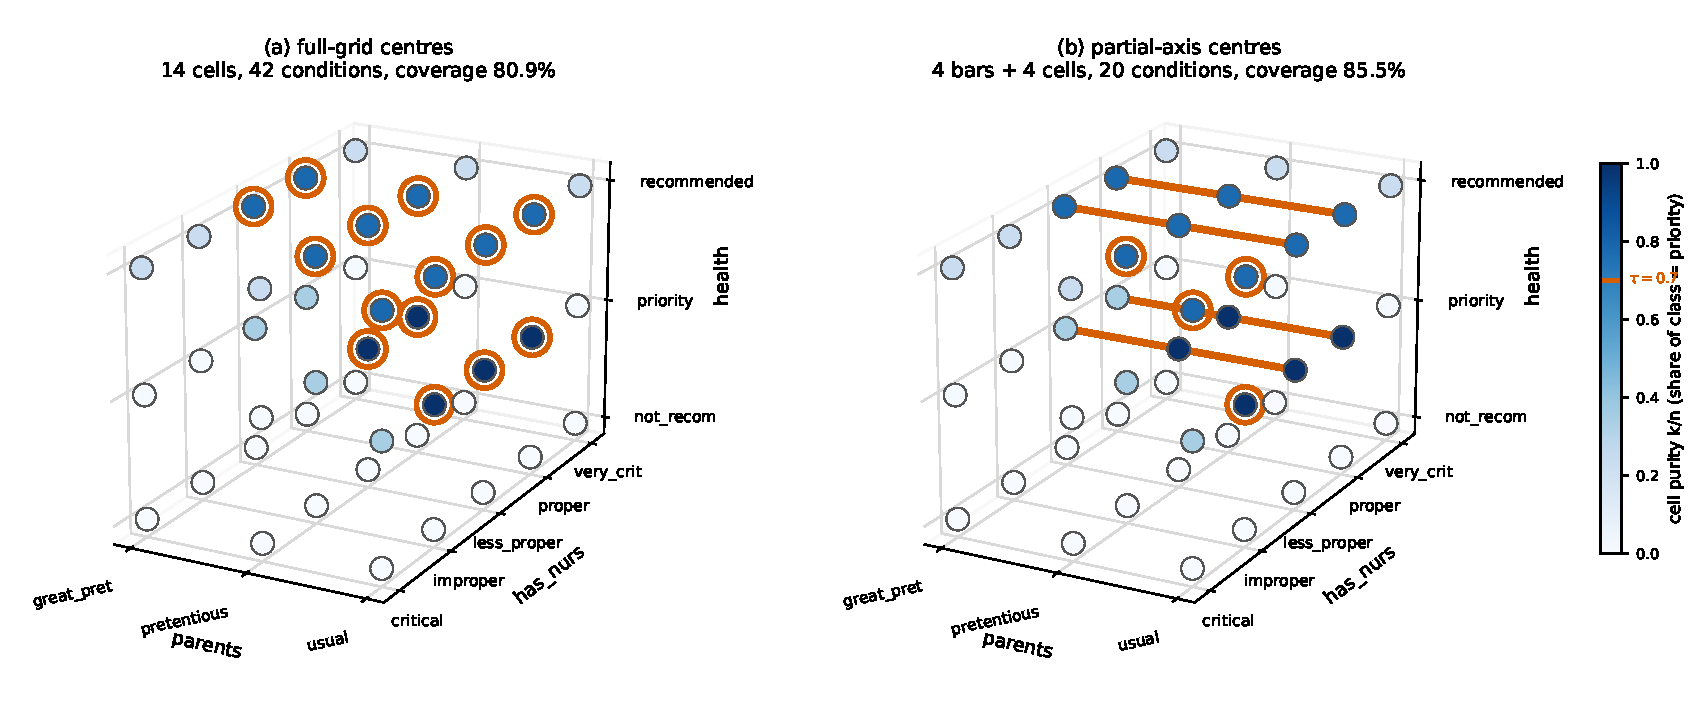
\includegraphics[width=\linewidth]{fig_example.pdf}
\caption{Выигравшая схема $\texttt{parents}\times\texttt{has\_nurs}\times\texttt{health}$ на \texttt{nursery} ($\texttt{class}=\texttt{priority}$, $\tau=0{,}7$, $m=1$, все строки; \texttt{experiments/fig\_example.py}). Сферы~--- 45 занятых ячеек, окрашенных по чистоте $k/n$ (метка на цветовой шкале~--- $\tau$). (a) Полная сетка: 14 ячеек с чистотой $\ge\tau$ обведены. (b) Центры на части осей: четыре стержня, каждый~--- ячейка подсетки $\texttt{has\_nurs}\times\texttt{health}$, проведённая через три входящие в неё ячейки вдоль свободной оси \texttt{parents}, и четыре полные ячейки. Числа~--- в разделе~\ref{sec:partial}. (Надписи на самом рисунке оставлены на английском.)}\label{fig:example}
\end{figure}

\begin{figure}[t]\centering
\begin{tikzpicture}[scale=0.62,every node/.style={font=\scriptsize}]
\begin{scope}
\draw[step=1,gray!60] (0,0) grid (3,3);
\fill[red!45] (0,0) rectangle (1,3); \draw[gray!60] (0,1)--(1,1) (0,2)--(1,2);
\node at (1.5,-0.55) {$A$}; \node at (-0.5,1.5) {$B$};
\node[align=center] at (1.5,-1.6) {три полные ячейки\\ $3\times2=6$ условий};
\end{scope}
\begin{scope}[xshift=5.5cm]
\draw[step=1,gray!60] (0,0) grid (3,3);
\fill[red!45] (0,0) rectangle (1,3); \draw[red!70!black,very thick] (0,0) rectangle (1,3);
\node at (1.5,-0.55) {$A$}; \node at (-0.5,1.5) {$B$};
\node[align=center] at (1.5,-1.6) {один частичный центр $A{=}a_1$\\ $1$ условие};
\end{scope}
\begin{scope}[xshift=11cm]
\draw[gray!60] (0,0) grid (3,3);
\draw[gray!60] (3,0)--(4.2,0.9)--(4.2,3.9)--(3,3); \draw[gray!60] (0,3)--(1.2,3.9)--(4.2,3.9);
\fill[red!45,opacity=.85] (0,0) rectangle (1,3);
\fill[blue!35,opacity=.75] (0,2)--(3,2)--(4.2,2.9)--(1.2,2.9)--cycle;
\node at (1.5,-0.55) {$A$}; \node at (-0.5,1.5) {$B$}; \node at (4.05,0.35) {$C$};
\node[align=center] at (2.1,-1.6) {стержень $A{=}a_1$ и пластина $B{=}b_3$\\ на одном кубе: $2$ условия};
\end{scope}
\end{tikzpicture}

\caption{Почему фиксация каждой оси стоит условий (схема; закрашенные области~--- входящие ячейки, которые программа рисует линией через них). Слева: на сетке $(A,B)$ группа $A{=}a_1$~--- это три полные ячейки, шесть условий. В центре: та же группа как один частичный центр, одно условие; на отображении $(A,B)$ это стержень. Справа: две группы по разным столбцам одной четырёхстолбцовой схемы~--- это стержень и пластина одного куба, два условия; как полные ячейки четырёхстолбцовой сетки они составили бы $9+9$ ячеек по четыре условия каждая.}\label{fig:mech}
\end{figure}

При бюджете в $B$ условий (раздел~\ref{sec:protocol}) упаковка превращается в задачу бюджетного максимального покрытия по непересекающимся кандидатам; мы используем жадный алгоритм по эффективности затрат с ленивым вычислением, сравниваемый с лучшим одиночным доступным по бюджету кандидатом~\citep{khuller1999}, ограниченный кандидатами, не пересекающимися с уже выбранными. Обе упаковки эвристические, и поиск по одной сетке тоже выбирает схему по результату жадного алгоритма. В разделе~\ref{sec:packing} обе задачи решаются точно на малых таблицах исследования, как целочисленные программы над теми же кандидатами и фолдами: на 540 ячейках (конфигурация, разбиение, бюджет) каждая программа решена до оптимальности, и жадный алгоритм в среднем отстаёт от оптимума на $0{,}01$ пункта покрытия под сертификатом и на $0{,}6$ пункта по правилу наблюдаемой чистоты~--- меньше, чем те $1{,}0$ пункта, которых тот же жадный алгоритм стоит свободным непересекающимся правилам.

На рис.~\ref{fig:example} показана одна выигравшая схема с частичными центрами на \texttt{nursery}: сетка $\texttt{parents}\times\texttt{has\_nurs}\times\texttt{health}$ имеет 45 занятых ячеек по 288 строк (таблица~--- полный факторный план, так что размер ничего не кодирует); 14 из них достигают $\tau=0{,}7$ и покрывают $80{,}9\,\%$ целевой переменной за 42 условия, тогда как четыре стержня подсетки $\texttt{has\_nurs}\times\texttt{health}$ (например, $\texttt{has\_nurs}=\texttt{less\_proper}\wedge\texttt{health}=\texttt{priority}$: $675$ из $864$ строк, чистота $0{,}78$, два условия) и четыре полные ячейки покрывают $85{,}5\,\%$ за 20. Стержень объединяет ячейки, которые по отдельности выше и ниже $\tau$, в группу, которая выше,~--- ячейка полной сетки этого сделать не может.

\subsection{Что показывает отображение}\label{sec:display}
Инструмент рисует выигравшую схему каждой размерности в виде решётки: одна отметка на каждую занятую ячейку сетки, независимо от того, является ли ячейка центром. Размер отметки~--- число строк ячейки; её цвет~--- доля целевой переменной в ячейке, в трёх зонах, заданных двумя порогами, которые по умолчанию равны базовой доле и $\tau$: не выше базовой доли, между ними и не ниже $\tau$ (центры). По запросу отметка сообщает своё число, свою долю и точный биномиальный интервал для доли. Частичные центры рисуются линиями или пластинами через входящие в них ячейки и перечисляются рядом с решёткой, каждый со своими условиями, числом, долей и интервалом. Панель перечисляет выигравшую схему каждой размерности с её покрытием, числом центров и потраченными на них условиями, так что цена ещё одного столбца видна на экране. Сдвиг $\tau$ перезапускает поиск, поскольку лучшая схема зависит от порога. На экране доступны оба правила отбора вместе с порогом размера $m$: по правилу наблюдаемой чистоты каждый центр показан со своим интервалом, а по сертифицированному правилу из раздела~\ref{sec:certificate} центрами являются только ячейки, прошедшие семейный порог, так что центры, показанные после сдвига порога, несут гарантию теоремы~\ref{thm:cert} без дополнительной поправки.

Помимо решётки, интерфейс имеет ещё пять представлений того же анализа: каждая оценённая схема одной размерности, размещённая по своему покрытию и числу центров, так что победитель виден среди альтернатив; покрытие и число центров лучшей схемы при каждом пороге с шагом в целый процент, по одной кривой на размерность; ячейки выигравших схем в виде списка правил, который можно фильтровать по условию; для каждого центра~--- другие описания, выбирающие те же или почти те же строки; и обзор одних столбцов (пары, почти определяющие друг друга, доминирующие уровни и уровни-заглушки), вычисляемый до выбора целевой переменной.

\begin{table}[t]\centering\footnotesize\setlength{\tabcolsep}{4pt}
\caption{Что содержит каждый вывод, исходя из его определения. Это свойства выводов, а не измерения того, насколько хорошо люди их читают. «Свободные правила»~--- конъюнкции не более чем из четырёх условий из раздела~\ref{sec:protocol}; «дерево»~--- дерево глубины~4, жадное или оптимальное.}\label{tab:properties}
\begin{tabular}{>{\raggedright\arraybackslash}p{0.30\linewidth}>{\raggedright\arraybackslash}p{0.15\linewidth}>{\raggedright\arraybackslash}p{0.14\linewidth}>{\raggedright\arraybackslash}p{0.15\linewidth}>{\raggedright\arraybackslash}p{0.13\linewidth}}
\toprule
& решётка (эта статья) & свободные правила & дерево & список SSD++\\
\midrule
Порог чистоты $\tau$~--- параметр поиска & да & да & нет (CART); через веса классов (оптимальное) & нет\\
Сертификат после поиска, на всех строках & да & да & нет & нет\\
Сертификат сохраняется при последующем сдвиге $\tau$ & да & да & -- & --\\
Показаны строки вне выбранных групп & да, по каждой ячейке схемы & нет & да, по каждому листу & как одно правило по умолчанию\\
Выбранные группы не пересекаются & да & только если наложено & да & да (упорядоченно)\\
Сколько столбцов может назвать описание & не более 4 & растёт с бюджетом & до 15 & растёт со списком\\
\bottomrule
\end{tabular}
\end{table}

В таблице~\ref{tab:properties} эти свойства сопоставлены с выводами базовых методов. Две её строки~--- то, чего сравнение в разделе~\ref{sec:results} показать не может. Список правил содержит выбранные группы и больше ничего: ячеек, не дотянувших до порога, и того, насколько не дотянувших, в нём нет, тогда как решётка и дерево учитывают каждую строку. А из двух выводов, учитывающих каждую строку, только решётка сопровождается порогом, который аналитик может двигать с сохранением гарантии; дерево строится без порога, и подсветка его листьев по порогу~--- фильтр, применяемый постфактум. Чего таблица не утверждает~--- что решётку легче читать. Трёхмерная решётка прячет отметки за отметками и кодирует числа размерами, которые считываются менее точно, чем напечатанные числа, а дерево печатает число и долю в каждом листе. Этот баланс мы не измеряли (раздел «Ограничения»).

\section{Сертификат, переживающий поиск}\label{sec:certificate}

Пусть $\mathcal{T}$~--- множество различных множеств строк среди занятых ячеек всех разбиений, которые может показать поиск: поискового разбиения каждой схемы с $|S|\le 4$ и, там где правило ёмкости слило уровни, также неслитого разбиения. $T=|\mathcal{T}|$ фиксировано, как только зафиксированы столбцы, и не зависит ни от целевой переменной, ни от $\tau$, ни от $m$.

\begin{theorem}[Сертификат с контролем групповой ошибки]\label{thm:cert}
Пусть при условии на столбцы строки независимы и $\Pr(z_i=1)=p_i$. Для ячейки $c$ со строками $I_c$ положим $\bar p_c=\frac1{n_c}\sum_{i\in I_c}p_i$~--- среднюю вероятность успеха строк, попавших в ячейку; именно об этой величине говорит сертификат. Пусть
\[
k^*(n,\tau,\lambda)=\min\Big\{k:\ k\ge\lceil n\tau\rceil+1,\ \Pr\big(\mathrm{Bin}(n,\tau)\ge k\big)\le\lambda\Big\}.
\]
Тогда при $\lambda=\alpha/T$ вероятность того, что некоторая ячейка $c\in\mathcal{T}$ с $\bar p_c\le\tau$ имеет $k_c\ge k^*(n_c,\tau,\lambda)$, не превосходит $\alpha$ одновременно для всех $\tau\in(0,1)$ и для любого правила, по которому схемы выбираются после просмотра целевой переменной.
\end{theorem}

\begin{proof}[Набросок доказательства]
$k_c$ имеет пуассон-биномиальное распределение со средним $n_c\bar p_c$. По теореме~4 Хёфдинга~\citep{hoeffding1956} при $k-1\ge n\bar p_c$ верхний хвост пуассон-биномиальной суммы не больше хвоста $\mathrm{Bin}(n,\bar p_c)$; порог определён как наименьшее $k^*$, для которого (i) $k^*\ge\lceil n\tau\rceil+1$ и (ii) $\Pr[\mathrm{Bin}(n,\tau)\ge k^*]\le\alpha/T$, так что $k^*-1\ge n\tau\ge n\bar p_c$ и сравнение применимо. В реализации (i) вычисляется в точной рациональной арифметике, а (ii)~--- на уровне $\lambda(1-10^{-9})$, так что ошибка округления с плавающей точкой в биномиальном хвосте может только отказать в сертификате, но никогда не выдать его. Условие (i) не косметическое: без него биномиальный тест антиконсервативен для гетерогенных строк ($n=3$, $\tau=0{,}01$, уровень $0{,}0298$: биномиальный порог равен $k=1$, а строки с $p=(0{,}03,0,0)$, среднее $0{,}01$, дают $\Pr[k\ge1]=0{,}03$~--- выше уровня; по неравенству о средних вероятность хотя бы одного успеха минимальна, когда все $p_i$ равны). Монотонность биномиального хвоста по $p$ даёт $\Pr(k_c\ge k^*)\le\Pr(\mathrm{Bin}(n_c,\tau)\ge k^*)\le\alpha/T$ для каждой ячейки с $\bar p_c\le\tau$. Оценка объединения по $T$ ячейкам, которые фиксированы при данных столбцах, даёт утверждение о групповой ошибке независимо от того, как была выбрана показанная схема. Одновременность по $\tau$: оба условия, определяющие $k^*$, монотонны, поэтому $k^*(n,\tau,\lambda)$ не убывает по $\tau$. Если ячейка со средним $\bar p_c$ сертифицирована при некотором $\tau'\ge\bar p_c$, то $k_c\ge k^*(n_c,\tau',\lambda)\ge k^*(n_c,\bar p_c,\lambda)$, и рассуждение выше, применённое при $\tau=\bar p_c$ (условие (i) выполнено для $k^*(n_c,\bar p_c,\lambda)$ по определению), ограничивает вероятность этого события величиной $\lambda$. Значит, для каждой ячейки есть одно событие вероятности не более $\lambda$, какое бы $\tau'$ ни выбрал аналитик после просмотра данных, и оценка объединения берётся по $T$ таким событиям.
\end{proof}

\paragraph{Оцениваемая величина.} Теорема ограничивает $\bar p_c$~--- среднее условных вероятностей успеха строк, оказавшихся в ячейке, при заданных всех столбцах. Это не утверждение о доле в генеральной совокупности $\Pr(z=1\mid\text{ячейка})$: популяционная версия потребовала бы, чтобы строки были выборкой из совокупности, и добавила бы изменчивость состава самой ячейки; она вне рамок статьи, и ничто ниже её не использует. На сгенерированной таблице (\texttt{nursery}, \texttt{mushroom}, таблицы эндшпилей) выборки нет вовсе, и сертификат~--- утверждение об условных вероятностях порождающей модели.

\paragraph{Что предполагает теорема.} Независимость строк при заданных столбцах. Положительно зависимые строки (члены одной семьи на \texttt{titanic}, которые склонны выжить или погибнуть вместе) делают число в ячейке более изменчивым, чем пуассон-биномиальная сумма с тем же средним, поэтому оценка хвоста больше не выполняется и уровень не гарантирован; из десяти конфигураций, сертифицирующих хоть что-то, \texttt{titanic}~--- та, где такая зависимость задокументирована, и её две сертифицированные ячейки (раздел~\ref{sec:intro-example})~--- те, для которых читателю следует соответственно скорректировать уровень. Семейство должно быть зафиксировано до чтения целевой переменной: в экспериментах разбиение на интервалы, правило ёмкости и набор столбцов не зависят от целевой переменной; в интерактивной программе обзор данных сообщает о проверке утечки после того, как названа целевая переменная, и пользователь, исключивший столбец на этом основании, сделал семейство зависящим от целевой переменной, поэтому выбранный так набор столбцов должен быть зафиксирован до рассмотрения следующего значения целевой переменной. Гарантия даётся на тройку (значение целевой переменной, направление, набор столбцов): аналитик, рассматривающий $V$ значений целевой переменной или и наличие, и отсутствие, запускает $V$ семейств и сохраняет уровень, деля $\alpha$ на $V$; программа этого за него не делает. Ресэмплинг Уэстфолла--Янга рассматривался и был отвергнут: перестановка целевой переменной проверяет независимость, а не $\bar p_c\le\tau$, и помечает ячейку чистоты $0{,}85$ как значимую при $\tau=0{,}9$ (\texttt{experiments/permutation\_null.py}: скорректированное $p<0{,}01$ в каждом запуске, сертификат пуст в каждом запуске). Приём Тароне удаляет ячейки, которые не могут достичь $k^*$, даже если целевое значение несёт каждая строка. Наименьшее $p$-значение, достижимое ячейкой из $n$ строк при пороге $\tau$, равно $\tau^n$ и растёт с $\tau$, поэтому ячейка, непроверяемая при $\tau_0$, непроверяема и при любом $\tau\ge\tau_0$, и сокращённое семейство, вычисленное при $\tau_0$, сохраняет гарантию одновременно для всех $\tau\ge\tau_0$; теряются только пороги ниже $\tau_0$. Здесь два условия. $\tau_0$ должен фиксироваться без целевой переменной: естественный выбор, базовая доля $P/N$, вычисляется по целевой переменной и делает семейство зависящим от неё. И выигрыш мал: наименьшая сертифицируемая ячейка уменьшается лишь логарифмически: на \texttt{titanic} при $\tau=0{,}9$ лишь $K=314$ из $T=3\,102$ множеств строк достаточно велики, чтобы достичь порога на уровне $\alpha/K$, и $n_{\min}$ падает с $105$ до $84$ для чистой ячейки и с $542$ до $405$ при чистоте $0{,}95$ (\texttt{experiments/n\_min\_table.py}; $K$~--- наименьшее $K$, при котором проверяемых множеств не более $K$, найденное бисекцией). Столбцы с редукцией Тароне приведены рядом с семейной оценкой в таблице~\ref{tab:nmin}; раздел~\ref{sec:taucurve} сравнивает их по всему диапазону порогов.

\paragraph{Почему оценка объединения.} Семейство~--- это множество различных множеств строк, а не описаний, и это уже наименьшее семейство, к которому можно привязать отображение: две ячейки с одинаковыми строками~--- одна гипотеза, а ячейка, которую поиск может показать, но которой нет в семействе, была бы гипотезой без бюджета ошибки. Среди поправок над этим семейством оценка мультипликативного типа (Шидак) или пошаговая процедура, предполагающая положительную зависимость, неприменимы: ячейки разных разбиений пересекаются всеми способами, которые допускают столбцы,~--- двумерная ячейка содержит трёхмерные, две двумерные ячейки на разных парах столбцов пересекаются,~--- и их пуассон-биномиальные числа такой структуры не имеют. Пошаговая процедура Холма корректна при произвольной зависимости и никогда не слабее оценки объединения, и в таблице~\ref{tab:counts} она используется для парных сравнений; для сертификата она не используется по двум причинам. Её решение для одной ячейки зависит от упорядоченных $p$-значений всех остальных ячеек, поэтому у ячейки больше нет собственного порога $k^*(n_c,\tau,\alpha/T)$, и одновременность по интерактивному $\tau$ теряется; а её выигрыш над Бонферрони~--- это число отклонений относительно $T$, то есть здесь горстка против тысяч. Выигрыш любой поправки ограничен: оценка объединения по $T$ стоит $\log T$ в пороге, и таблица~\ref{tab:nmin} показывает, что от $T=2\,100$ до $T=7\,282\,600$ наименьшая сертифицируемая ячейка растёт в $1{,}8$ раза; поправка, точная для зависимости, сэкономила бы часть этого множителя и ничего из цены чистоты, а именно там сертификат дорог.

\paragraph{Цена.} В таблице~\ref{tab:nmin} приведено $n_{\min}$~--- наименьшая ячейка, которую сертификат может сертифицировать при $\alpha=0{,}05$,~--- для ячейки, все строки которой несут целевое значение, и для ячейки с наблюдаемой чистотой на пять пунктов выше $\tau$, как функция размера семейства $T$ (\texttt{experiments/certificate\_price.py}~--- реализация порога на стандартной библиотеке, воспроизводящая перебор на scipy из \texttt{n\_min\_table.py} в каждой строке). От $M=5$ до $M=30$ столбцов $T$ растёт в $3\,500$ раз, а $n_{\min}$~--- в $1{,}8$ раза: цена поиска логарифмична по семейству. Цена чистоты~--- нет: запас в пять пунктов требует $1\,400$--$2\,600$ строк при $\tau=0{,}7$ и $500$--$1\,000$ при $\tau=0{,}9$ при любом $M$, так что на таблицах из нескольких сотен строк сертификат не сертифицирует ничего, кроме чистых ячеек, а при $\tau=0{,}9$~--- ничего на \texttt{titanic}. В той же таблице рядом с семейной оценкой стоит разбиение на исследовательскую и контрольную части~\citet{webb2007}: разбиение проверяет только $T_B$ кандидатов, которые предлагает половина~A, но на половине строк, поэтому ячейка должна быть в таблице примерно вдвое больше, чем ей нужно в половине~B. По этому расчёту при $T_B=10$ кандидатах разбиению нужны примерно те же ячейки, что и семейной оценке по $3\,102$ множествам строк ($30$ против $31$ строки для чистой ячейки, $1\,122$ против $1\,425$ при запасе в пять пунктов; больше при большем $T_B$), и его ответ зависит от случайного деления строк, а ответ семейной оценки~--- нет. Следующий абзац показывает, что на данных этот расчёт приукрашивает разбиение.

\begin{table}[t]\centering\footnotesize\setlength{\tabcolsep}{3.5pt}
\caption{Наименьшая сертифицируемая ячейка $n_{\min}$ при $\alpha=0{,}05$, чистая / наблюдаемая чистота $\tau+0{,}05$, для семейного сертификата ($T$ различных множеств строк по $d\le4$ на всех строках) и для разбиения на исследовательскую и контрольную части с $T_B$ кандидатами (строк во всей таблице, вдвое больше, чем нужно половине~B). Получено \texttt{experiments/certificate\_price.py}.}\label{tab:nmin}
\begin{tabular}{lrrrrrrr}
\toprule
& & \multicolumn{2}{c}{семейство} & \multicolumn{2}{c}{семейство, Тароне} & \multicolumn{2}{c}{разбиение, $T_B=10$}\\
данные & $T$ & $\tau=0{,}7$ & $\tau=0{,}9$ & $\tau=0{,}7$ & $\tau=0{,}9$ & $\tau=0{,}7$ & $\tau=0{,}9$\\
\midrule
синтетика ($N=5\,000$, $M=5$) & 2\,100 & 30 / 1365 & 102 / 508 & 28 / 1229 & 85 / 407 & 30 / 1122 & 102 / 444\\
titanic ($N=891$, $M=8$) & 3\,102 & 31 / 1425 & 105 / 542 & 28 / 1229 & 84 / 405 & 30 / 1122 & 102 / 444\\
car\_evaluation ($N=1\,728$, $M=6$) & 3\,391 & 32 / 1437 & 106 / 544 & 28 / 1249 & 79 / 384 & 30 / 1122 & 102 / 444\\
nursery ($N=12\,960$, $M=8$) & 11\,030 & 35 / 1621 & 117 / 606 & 35 / 1621 & 110 / 566 & 30 / 1122 & 102 / 444\\
mushroom ($N=8\,124$, $M=21$) & 49\,254 & 39 / 1853 & 131 / 688 & 38 / 1789 & 122 / 643 & 30 / 1122 & 102 / 444\\
синтетика ($N=5\,000$, $M=10$) & 62\,200 & 40 / 1889 & 134 / 706 & 34 / 1581 & 95 / 467 & 30 / 1122 & 102 / 444\\
chess\_krkp ($N=3\,196$, $M=36$) & 303\,620 & 44 / 2137 & 149 / 803 & 44 / 2105 & 144 / 766 & 30 / 1122 & 102 / 444\\
синтетика ($N=5\,000$, $M=20$) & 1\,316\,400 & 48 / 2365 & 163 / 884 & 40 / 1921 & 106 / 543 & 30 / 1122 & 102 / 444\\
синтетика ($N=5\,000$, $M=30$) & 7\,282\,600 & 53 / 2637 & 179 / 984 & 44 / 2117 & 113 / 584 & 30 / 1122 & 102 / 444\\
\bottomrule
\end{tabular}

\end{table}

\paragraph{Против контрольного разбиения на данных.} Таблица~\ref{tab:split} (приложение~\ref{app:tables}) запускает разбиение на исследовательскую и контрольную части~\citet{webb2007} на тех же фолдах, что и семейный сертификат (раздел~\ref{sec:protocol}: половина~A обучающего фолда предлагает группы по правилу наблюдаемой чистоты, половина~B проверяет каждую предложенную группу один раз на уровне $\alpha/T_B$, где $T_B$~--- число различных групп, предложенных по шести бюджетам). Расчёт выше, давший обоим сертификатам одинаковое $n_{\min}$ при $T_B=10$,~--- не то, что происходит: на десяти конфигурациях, сертифицирующих что-либо по семейной оценке, частичные центры, сертифицированные разбиением, покрывают меньше в девяти (в среднем $31$ против $40$ пунктов при $B=32$), а на пяти, не сертифицирующих ничего по семейной оценке, разбиение сертифицирует несколько пунктов, чистота которых на отложенных строках редко достигает $\tau$ (таблица~\ref{tab:split}). Это объясняют две вещи, которые расчёт упустил. Предлагающая половина видит половину строк, поэтому ячейки, проходящие порог размера и правило чистоты на полном обучающем фолде, не обязаны проходить их на его половине; и $T_B$ считает каждое различное предложение каждого бюджета, а не десять. Разбиение~--- корректный сертификат для всех методов одинаково, включая дерево, и в этом его единственное преимущество здесь; сертифицирует же оно мелкие ячейки, близкие к $\tau$: чистота объединения, сертифицированного разбиением, на отложенных строках достигает $\tau$ в $49\,\%$ разбиений для частичных центров против $97\,\%$ при семейной оценке. Семейная оценка проверяет больше гипотез на более строгом уровне, но на всех строках, и на этих таблицах такой обмен выгоднее.

\paragraph{Мощность.} Рис.~\ref{fig:power} даёт вероятность того, что ячейка из $n$ строк, каждая из которых несёт целевое значение с вероятностью $p$, будет сертифицирована; таблица~\ref{tab:n80}~--- размер, при котором эта вероятность достигает $0{,}8$. Чистая ячейка сертифицируется почти наверняка, как только превышает $n_{\min}$; ячейке с $p=\tau+0{,}05$ нужно примерно $1{,}4\times n_{\min}$ строк ($2\,020$ при $\tau=0{,}7$, $729$ при $\tau=0{,}9$ для семейства \texttt{titanic}). В симуляции \texttt{experiments/certificate\_power.py} (восемь трёхуровневых столбцов, истинный центр с чистотой $0{,}95$, ячейка ровно с $\tau=0{,}8$, фон $0{,}10$) мощность при строгом контроле равна 1\,\% при $N=500$, 57\,\% при $N=1\,000$, 99,5\,\% при $N=2\,000$ и 100\,\% от $N=5\,000$ до $N=20\,000$ (200 запусков на размер), при одном ложном сертификате на $1\,200$ запусков~--- на граничной ячейке; посхемный сертификат, который продукт использовал раньше, имеет мощность 0,75 при $N=500$, но групповую частоту ложных сертификатов 67\,\% на чистом шуме при $d\le4$ (1\,000 запусков; 95\%-й интервал $64$--$70\,\%$), тогда как семейный сертификат не делает ни одного на $1\,000$ запусков, так что его частота на чистом шуме ниже $0{,}4\,\%$ с доверием $95\,\%$ (\texttt{experiments/null\_certificate.py}). В исследовании сертификат непуст на 10 из 19 реальных конфигураций (раздел~\ref{sec:results}); стоит ли он своей цены~--- вопрос $N$, $\tau$ и запаса, и ответ на него~--- таблица~\ref{tab:n80} и кривая выше.

\begin{figure}[t]\centering
% Generated data: fig_certificate_power.dat (experiments/certificate_price.py).
\begin{tikzpicture}
\begin{groupplot}[group style={group size=2 by 1, horizontal sep=14mm},
  width=0.5\linewidth, height=0.36\linewidth, xmode=log, ymin=0, ymax=1.02,
  xmin=10, xmax=3000, xlabel={размер ячейки $n$}, grid=major, grid style={gray!25},
  tick label style={font=\scriptsize}, label style={font=\scriptsize}, title style={font=\small},
  legend style={font=\scriptsize, draw=none, fill=white, fill opacity=0.85, text opacity=1,
                at={(0.03,0.97)}, anchor=north west, cells={anchor=west}}]
\nextgroupplot[title={$\tau=0{,}7$}, ylabel={$\Pr[\text{сертиф.}]$}]
\addplot[black, thick] table[x=n, y=titanic_t70_p100] {fig_certificate_power.dat};
\addplot[black, thick, dashed] table[x=n, y=chess_t70_p100] {fig_certificate_power.dat};
\addplot[red!70!black, thick] table[x=n, y=titanic_t70_p75] {fig_certificate_power.dat};
\addplot[red!70!black, thick, dashed] table[x=n, y=chess_t70_p75] {fig_certificate_power.dat};
\nextgroupplot[title={$\tau=0{,}9$}]
\addplot[black, thick] table[x=n, y=titanic_t90_p100] {fig_certificate_power.dat};
\addlegendentry{$p=1$, $T=3\,102$}
\addplot[black, thick, dashed] table[x=n, y=chess_t90_p100] {fig_certificate_power.dat};
\addlegendentry{$p=1$, $T=303\,620$}
\addplot[red!70!black, thick] table[x=n, y=titanic_t90_p95] {fig_certificate_power.dat};
\addlegendentry{$p=\tau+0{,}05$, $T=3\,102$}
\addplot[red!70!black, thick, dashed] table[x=n, y=chess_t90_p95] {fig_certificate_power.dat};
\addlegendentry{$p=\tau+0{,}05$, $T=303\,620$}
\end{groupplot}
\end{tikzpicture}

\caption{Вероятность того, что ячейка из $n$ строк с вероятностью целевого значения $p$ в каждой строке будет сертифицирована при $\alpha=0{,}05$, для размеров семейств \texttt{titanic} ($T=3\,102$) и \texttt{chess} ($T=303\,620$). Однородные строки~--- случай, для которого порог точен.}\label{fig:power}
\end{figure}

\begin{table}[t]\centering\small
\caption{$n_{80}$: размер ячейки, при котором вероятность сертификации достигает $0{,}8$, рядом с $n_{\min}$ (таблица~\ref{tab:nmin}).}\label{tab:n80}
\begin{tabular}{llrrrr}
\toprule
$T$ & $\tau$ & $p=\tau+0{,}05$ & $p=1$ & \multicolumn{2}{l}{$n_{\min}$ (чистая / $\tau+0{,}05$)}\\
\midrule
3\,102 (titanic) & 0{,}7 & 2020 & 31 & 31 & 1425\\
3\,102 (titanic) & 0{,}9 & 729 & 105 & 105 & 542\\
303\,620 (chess) & 0{,}7 & 2856 & 44 & 44 & 2137\\
303\,620 (chess) & 0{,}9 & 1031 & 149 & 149 & 803\\
\bottomrule
\end{tabular}

\end{table}

\section{Протокол оценки}\label{sec:protocol}

\paragraph{Фолды.} Повторная стратифицированная $K$-кратная кросс-валидация ($5\times5$; $5\times3$ для \texttt{chess} и \texttt{splice}, $5\times2$ для \texttt{mushroom} и \texttt{adult} и $5\times1$ для \texttt{connect\_4}, где один повтор~--- это то, что позволил бюджет), одинаковая для всех методов, чтобы разности были парными. На \texttt{connect\_4} $t$-статистика Надо--Бенжио имеет четыре степени свободы (14 на \texttt{chess} и \texttt{splice}), так что отметка там~--- более слабое свидетельство, чем в других местах; $p$-значения за столбцами Холма в таблице~\ref{tab:counts} используют число степеней свободы каждой таблицы. Каждая подбираемая величина~--- интервалы фиксированы, но правило ёмкости, слияние уровней и размер семейства $T$~--- вычисляется на обучающем фолде; выбранные группы переносятся на отложенные строки через подобранное разбиение (невиданные уровни идут в группу «прочее»).

\paragraph{Выбор $\tau$ и $m$.} Порог чистоты каждой конфигурации задан вручную из сетки $\{0{,}3;\ 0{,}5;\ 0{,}7;\ 0{,}9\}$, когда её таблица вошла в исследование; он не следует одному правилу. Цель~--- порог существенно выше базовой доли, чтобы центр был концентрацией целевой переменной, а не пересказом базовой доли: $\tau$ лежит между $1{,}4$ и $5{,}0$ базовых долей и не меньше удвоенной базовой доли на 17 из 21 конфигурации (таблица~\ref{tab:data}); четыре исключения~--- \texttt{titanic} при $\tau=0{,}7$ и три целевых значения с базовой долей около половины или выше (\texttt{mushroom}, \texttt{chess}, \texttt{connect\_4} с целевым значением \texttt{win}), где $\tau=0{,}9$~--- верх сетки. Порог размера принимает два значения: $m=1$ на таблицах UCI и клинических, где это значение продукта по умолчанию, и $m=20$ на семи внешних таблицах с $N\ge1\,470$ и двух таблицах PMLB, где при $m=1$ свободные правила выбирают чистые на обучении ячейки из нескольких строк (раздел~\ref{sec:net}). \texttt{titanic} запускается при $\tau=0{,}9$ и $0{,}7$, а при $\tau=0{,}9$~--- с обоими порогами размера, и выводы при каждом одинаковы (таблицы~\ref{tab:purity32} и~\ref{tab:cert32}); \texttt{nursery} и \texttt{connect\_4} запускаются каждая для двух целевых значений, каждое с одним порогом. Список конфигураций хранится вместе с кодом, и история репозитория показывает, что ни у одной конфигурации $\tau$ или $m$ не менялись после коммита, который её ввёл. Поскольку пороги заданы вручную, сравнение методов на сетках и на правилах по наблюдаемой чистоте повторено на одной фиксированной сетке $(\tau,m)$ для каждой таблицы (раздел~\ref{sec:grid}); что там не повторялось, сказано в разделе «Ограничения».

\paragraph{Бюджет.} Все методы отвечают на один вопрос: какие группы строк, не более чем из $B\in\{1,2,4,8,16,32\}$ условий, содержат больше всего положительных строк, если каждая имеет чистоту на обучении $\ge\tau$ (или сертифицирована семейной оценкой, или предложена на половине обучающего фолда и сертифицирована на другой половине) и размер $\ge m$? Ячейка $d$-столбцовой сетки стоит $d$; правило длины $\ell$ стоит $\ell$; лист дерева стоит свою глубину.

\paragraph{Методы.}
\texttt{vsf}: лучшая схема для бюджета, её $\lfloor B/d\rfloor$ лучших центров.
\texttt{vsf\_partial}: лучшая схема для бюджета с частичными центрами, непересекающийся жадный алгоритм.
\texttt{vsf\_greedy}: вложенная цепочка $S_1\subset S_2\subset S_3\subset S_4$ (тот жадный подход, против которого выступает исчерпывающий поиск).
\texttt{rules}: каждая конъюнкция из $\le 4$ условий, встречающаяся в обучающих строках, бюджетное максимальное покрытие (могут пересекаться).
\texttt{rules\_pure}: \texttt{rules}, где объединение удерживается при чистоте на обучении $\ge\tau$.
\texttt{rules\_disjoint}: \texttt{rules} без общих обучающих строк.
\texttt{tree}: CART на one-hot столбцах, лучший по глубине $\le 4$, критерию и весу класса; подходящие листья~--- тем же жадным алгоритмом. По сертифицированному правилу листья дерева не являются заранее заданным семейством, так что фильтр~--- только фильтр, а не сертификат (см. ниже).
\texttt{wracc}: подходящее семейство \texttt{rules}, ранжированное по взвешенной относительной точности $\mathrm{WRAcc}=\frac{n}{N}\big(\frac{k}{n}-\frac{P}{N}\big)$~--- стандартному качеству поиска подгрупп (pysubgroup, SD-Map, CN2-SD),~--- читаемое как список top-$k$: правила берутся в этом порядке, пока помещаются в бюджет, пересечения допускаются. Это то, что возвращает «инструмент поиска подгрупп с фильтром чистоты».
\texttt{wracc\_raw}: тот же список без фильтра чистоты (только размер $\ge m$, 256 лучших ячеек по WRAcc): то, что инструмент возвращает «из коробки». Не решение задачи; оставлено, чтобы показать, что меняет порог чистоты.
\texttt{tree\_opt}: оптимальное дерево (DL8.5,~\citealp{aglin2020}; пакет \texttt{pydl8.5}) глубины $\le d$ для каждого $d\le4$ на one-hot столбцах, минимизирующее взвешенную по классам ошибку с весами $1:\tau/(1-\tau)$, оптимум которой по листьям~--- чистое покрытие; веса реализованы размножением строк (при $\tau=0{,}7$ положительные трижды, отрицательные семь раз), так что поиск точен и не требует обратного вызова. Далее листья обрабатываются в точности как у CART. Запускается на всех 17 таблицах; на \texttt{adult} ни одна подгонка не упёрлась в десятиминутный лимит (0\,\% таймаутов в таблице~\ref{tab:treeopt}), тогда как на \texttt{connect\_4} подгонки упирались в лимит на 40--100\,\% разбиений (таблица~\ref{tab:treeopt}). На остальных таблицах ни одна подгонка не упёрлась в десятиминутный лимит.
\texttt{ssdpp}: SSD++~\citep{proenca2022}~--- MDL-список правил, подгоняемый на обучающем фолде для двухклассовой целевой переменной (луч 30, не более 40 правил, глубина $\le4$, минимальная поддержка $m$); список правил упорядочен, так что его $i$-е правило применяется к строкам, которые не подошли ни под одно более раннее правило, и его группы не пересекаются по построению. Его подходящие правила входят в тот же бюджетный жадный алгоритм со стоимостью, равной числу условий. Это сильнейший опубликованный метод поиска наборов подгрупп с контролем избыточности; его цель (сжатие всего столбца целевой переменной) отличается от нашей, и список содержит также правила для другого класса, которые никогда не подходят. Релиз пакета на PyPI требует патча совместимости с текущими numpy/pandas, который мы поставляем и применяем детерминированно.

\paragraph{Сертифицированный отбор для базовых методов.} По сертифицированному правилу каждый метод допускает группу по одному и тому же порогу $k^*(n,\tau,\alpha/T)$, где $T$~--- семейство из раздела~\ref{sec:certificate}, вычисленное на обучающем фолде. Для \texttt{rules}, \texttt{rules\_pure} и \texttt{rules\_disjoint} это корректный сертификат после отбора, а не просто тот же фильтр: конъюнкция из $\ell\le4$ условий на столбцах $S$, встречающаяся в обучающих строках,~--- это занятая ячейка разбиения $S$ (неслитого разбиения там, где правило ёмкости слило уровни), так что её множество строк~--- элемент $\mathcal{T}$, и семейство кандидатов базового метода на правилах совпадает с семейством поиска по сеткам. То же верно для \texttt{vsf\_greedy}. Для дерева и для SSD++ это только фильтр: лист выращивается по целевой переменной, а $i$-е правило списка применяется к остатку после первых $i-1$, который не является ячейкой никакого разбиения.

\paragraph{Метрики.} На отложенных строках: покрытие $k/P$ объединения выбранных групп; чистота $k/n$ объединения; чистое покрытие $(k-\frac{\tau}{1-\tau}(n-k))/P$~--- лагранжиан покрытия при ограничении чистоты $\ge\tau$; доля разбиений с чистотой на отложенных строках $\ge\tau$; стабильность описания (среднее попарное сходство Жаккара выбранных множеств строк по разбиениям); фактически потраченные условия; время отбора. Парные разности с поправленной дисперсией Надо--Бенжио~\citep{nadeau2003}. Инференциальное утверждение~--- столбец Холма в таблице~\ref{tab:counts}: ячейки, двустороннее $p$-значение которых выдерживает поправку Холма по бюджетам той же конфигурации на уровне $0{,}05$. Описательная отметка $|t|\ge2$ в остальных таблицах сохранена, поскольку именно её несут таблицы по бюджетам; это не тест фиксированного уровня (двусторонний $0{,}057$ при $24$ степенях свободы, $0{,}12$ при $4$), и каждый приведённый по ней подсчёт дан также после поправки Холма. Победы и поражения считаются по ячейкам (конфигурация, бюджет) и читаются как описательные подсчёты: шесть бюджетов одной конфигурации используют одни и те же разбиения и не независимы, а поправка не охватывает разные конфигурации; поэтому в разделе~\ref{sec:mechanism} каждый подсчёт приводится также при единственном бюджете $B=32$, по одной ячейке на конфигурацию.

\paragraph{Зачем непересекающийся базовый метод.} По правилу наблюдаемой чистоты чистота объединения \texttt{rules} на отложенных строках достигает $\tau$ в 60\,\% разбиений против 77--79\,\% для \texttt{vsf}, \texttt{vsf\_partial} и \texttt{rules\_disjoint} (таблица~\ref{tab:counts}; независимая реимплементация из раздела~\ref{sec:results} дала 53 против 73\,\%). Каждое правило имеет чистоту $\ge\tau$ на обучающих строках; их объединение~--- нет, поскольку правила пересекаются на строках, несущих целевое значение, а не на остальных. Поэтому сравнение одного лишь покрытия между пересекающимся и непересекающимся методами сравнивает разные ограничения.

\section{Данные}\label{sec:data}
Семнадцать реальных таблиц с закреплёнными хешами SHA-256 и зафиксированной предобработкой (таблица~\ref{tab:data}) и два дизайна с внедрённой структурой. Реальные таблицы дают 21 конфигурацию по правилу наблюдаемой чистоты: \texttt{titanic} входит трижды (одно целевое значение, два порога чистоты, два порога размера), а \texttt{nursery} и \texttt{connect\_4}~--- дважды каждая, каждый раз с другим целевым значением. Реальные таблицы~--- это классика поиска подгрупп из UCI (\texttt{mushroom}, \texttt{nursery}, \texttt{car}, \texttt{chess}), \texttt{titanic}, три небольшие клинические таблицы, две широкие таблицы PMLB (\texttt{connect\_4}, $67\,557\times42$; \texttt{splice}, $3\,188\times60$, где каждый метод ограничен $d\le3$, поскольку семейства размера~4 слишком велики для всех одинаково), семь таблиц из публичных зеркал с $N$ от 1\,470 до 48\,842 и базовыми долями от 8 до 28\,\% (\texttt{adult}, \texttt{hmda}, \texttt{credit}, \texttt{resume} и три таблицы поставщиков, являющиеся синтетическими или демонстрационными данными, а не наблюдениями: вымышленная \texttt{attrition} от IBM, демо \texttt{wa\_churn} от IBM и таблица \texttt{mlc\_churn}, которую пакет C5.0 описывает как искусственную). \texttt{car}, \texttt{nursery} (полные факторные планы из модели принятия решений), \texttt{chess} и \texttt{connect\_4} (перечисления эндшпилей) и \texttt{mushroom} (гипотетические образцы из полевого определителя) детерминированы или сгенерированы; наблюдательные таблицы~--- \texttt{adult}, \texttt{hmda}, \texttt{credit}, \texttt{resume}, \texttt{titanic}, \texttt{splice} и три клинические таблицы. Из десяти конфигураций, сертифицирующих хоть что-то, наблюдательные только \texttt{adult}, \texttt{hmda} и \texttt{titanic}. Внедрённые дизайны~--- \emph{выровненный} (одна 4-ячейка и одна 2-ячейка на одних и тех же четырёх столбцах) и \emph{невыровненный} (два правила из 2 условий на непересекающихся парах столбцов, которые никакая полная сетка из четырёх столбцов не может показать меньше чем $9+9$ ячейками). Три высокоразмерные таблицы экспрессии (325--7\,070 столбцов) есть в репозитории, но исключены: исчерпывающий поиск по $d\le4$ требует предварительного отбора признаков, который вошёл бы в семейство и сломал бы теорему~\ref{thm:cert}.

\begin{table}[t]\centering\footnotesize\setlength{\tabcolsep}{4pt}
\caption{Наборы данных и настройки, по строке на целевое значение (получено \texttt{experiments/paper\_tables.py} из манифеста и списка конфигураций). $\tau/\text{база}$~--- наименьшее отношение порога чистоты к базовой доле этого целевого значения.}\label{tab:data}
\begin{tabular}{lrrlrrl}
\toprule
набор & $N$ & $M$ & положит. значение & базовая доля & $\tau/\text{база}$ & $\tau$ / $m$ / повторы\\
\midrule
titanic & 891 & 8 & survived & 38\,\% & 1{,}8 & 0{,}7/1/5; 0{,}9/1/5; 0{,}9/20/5\\
breast\_cancer & 286 & 9 & recurrence-events & 30\,\% & 2{,}4 & 0{,}7/1/5\\
thyroid\_recurrence & 383 & 16 & Yes & 28\,\% & 3{,}2 & 0{,}9/1/5\\
breast\_cancer\_wisconsin & 699 & 9 & malignant & 34\,\% & 2{,}6 & 0{,}9/1/5\\
car\_evaluation & 1728 & 6 & acc & 22\,\% & 4{,}1 & 0{,}9/1/5\\
nursery & 12960 & 8 & spec\_prior & 31\,\% & 2{,}9 & 0{,}9/1/5\\
nursery & 12960 & 8 & priority & 33\,\% & 2{,}1 & 0{,}7/1/5\\
mushroom & 8124 & 21 & poisonous & 48\,\% & 1{,}9 & 0{,}9/1/2\\
chess\_krkp & 3196 & 36 & won & 52\,\% & 1{,}7 & 0{,}9/1/3\\
adult & 48842 & 12 & \textgreater{}50K & 24\,\% & 2{,}9 & 0{,}7/20/2\\
hmda & 2380 & 12 & yes & 12\,\% & 4{,}2 & 0{,}5/20/5\\
attrition & 1470 & 19 & Yes & 16\,\% & 3{,}1 & 0{,}5/20/5\\
credit & 4454 & 13 & bad & 28\,\% & 2{,}5 & 0{,}7/20/5\\
resume & 4870 & 24 & yes & 8\,\% & 3{,}7 & 0{,}3/20/5\\
wa\_churn & 7043 & 19 & Yes & 27\,\% & 2{,}6 & 0{,}7/20/5\\
mlc\_churn & 5000 & 11 & yes & 14\,\% & 5{,}0 & 0{,}7/20/5\\
connect\_4 & 67557 & 42 & loss & 25\,\% & 2{,}8 & 0{,}7/20/1\\
connect\_4 & 67557 & 42 & win & 66\,\% & 1{,}4 & 0{,}9/20/1\\
splice & 3188 & 60 & site\_b & 24\,\% & 3{,}7 & 0{,}9/20/3\\
\bottomrule
\end{tabular}

\end{table}

\section{Результаты}\label{sec:results}

\subsection{Цена одной сетки и её источник}\label{sec:mechanism}

\begin{table}[t]\centering\small
\caption{Парные сравнения по ячейкам (конфигурация, бюджет); неинформативные ячейки (ни один метод не превышает 1\,\% покрытия на отложенных строках) исключены. Слева: описательная отметка, $|t|\ge2$ по $t$-статистике Надо--Бенжио с $J-1$ степенями свободы ($J$ разбиений; двусторонний уровень около $0{,}06$ при $5\times5$ и $0{,}12$ при $5\times1$). Справа: ячейки, двустороннее $p$-значение которых выдерживает поправку Холма по информативным бюджетам той же конфигурации на уровне $0{,}05$. Ни одна поправка не охватывает разные конфигурации: это подсчёты ячеек, а не проверка одной глобальной гипотезы. Блок \emph{разбиение}~--- контрольный сертификат из раздела~\ref{sec:certificate}. «Закрытый разрыв»~--- $(\cov^{\mathrm{p}}-\cov)/(\cov_{\mathrm{rules\,disj}}-\cov)$ по ячейкам, где непересекающиеся правила превосходят сетку хотя бы на один пункт.}\label{tab:counts}
\begin{tabular}{llrrrrrr}
\toprule
& & \multicolumn{3}{c}{$|t|\ge2$} & \multicolumn{3}{c}{Холм внутри конфигурации}\\
отбор & сравнение & лучше & вровень & хуже & лучше & вровень & хуже\\
\midrule
сертиф. & полн.~сетка vs непер.~правила & 2 & 31 & 20 & 2 & 32 & 19\\
сертиф. & част.~центры vs непер.~правила & 2 & 45 & 6 & 2 & 48 & 3\\
сертиф. & част.~центры vs полн.~сетка & 18 & 35 & 0 & 15 & 38 & 0\\
сертиф. & \multicolumn{7}{l}{разрыв, закрытый част. центрами: медиана 1{,}00, среднее 0{,}86 ($n=21$)}\\
сертиф. & \multicolumn{7}{l}{чистота объедин. на отлож. $\ge\tau$: сетка 97\,\%, частичные 97\,\%, прав.$_{\mathrm{непер}}$ 97\,\%, правила 97\,\%}\\
\midrule
чистота & полн.~сетка vs непер.~правила & 2 & 62 & 45 & 1 & 66 & 42\\
чистота & част.~центры vs непер.~правила & 5 & 83 & 21 & 2 & 91 & 16\\
чистота & част.~центры vs полн.~сетка & 41 & 68 & 0 & 39 & 70 & 0\\
чистота & \multicolumn{7}{l}{разрыв, закрытый част. центрами: медиана 0{,}85, среднее 0{,}75 ($n=55$)}\\
чистота & \multicolumn{7}{l}{чистота объедин. на отлож. $\ge\tau$: сетка 79\,\%, частичные 79\,\%, прав.$_{\mathrm{непер}}$ 77\,\%, правила 60\,\%}\\
\midrule
разбиение & полн.~сетка vs непер.~правила & 1 & 70 & 7 & 1 & 72 & 5\\
разбиение & част.~центры vs непер.~правила & 3 & 75 & 0 & 3 & 75 & 0\\
разбиение & част.~центры vs полн.~сетка & 6 & 72 & 0 & 5 & 73 & 0\\
разбиение & \multicolumn{7}{l}{разрыв, закрытый част. центрами: медиана 0{,}98, среднее 0{,}87 ($n=30$)}\\
разбиение & \multicolumn{7}{l}{чистота объедин. на отлож. $\ge\tau$: сетка 43\,\%, частичные 49\,\%, прав.$_{\mathrm{непер}}$ 49\,\%, правила 50\,\%}\\
\bottomrule
\end{tabular}

\end{table}

\begin{table}[t]\centering\small
\caption{Покрытие на отложенных строках (\%) при $B=32$, отбор по наблюдаемой чистоте. Отметки: частичные центры против полной сетки (ч\,vs\,с) и против непересекающихся правил (ч\,vs\,п). У набора данных, запущенного для двух целевых значений или двух порогов размера, целевое значение или $m$ указаны в скобках.}\label{tab:purity32}
\begin{tabular}{llrrrrrcc}
\toprule
набор & $\tau$ & сетка & частичн. & прав.$_{\mathrm{непер}}$ & прав. & дерево & ч$\,$vs$\,$с & ч$\,$vs$\,$п\\
\midrule
titanic & 0{,}9 & 48 & 53 & 57 & 59 & 51 & + & -\\
titanic & 0{,}7 & 67 & 73 & 77 & 85 & 70 & + & -\\
titanic ($m{=}20$) & 0{,}9 & 47 & 46 & 47 & 53 & 47 & = & =\\
breast\_cancer & 0{,}7 & 27 & 32 & 39 & 49 & 30 & = & =\\
thyroid\_recurrence & 0{,}9 & 83 & 88 & 88 & 89 & 85 & = & =\\
breast\_cancer\_wisconsin & 0{,}9 & 82 & 85 & 75 & 94 & 89 & = & +\\
car\_evaluation & 0{,}9 & 21 & 21 & 12 & 12 & 0 & = & +\\
nursery (spec\_prior) & 0{,}9 & 42 & 57 & 59 & 68 & 28 & + & -\\
nursery (priority) & 0{,}7 & 63 & 86 & 87 & 90 & 67 & + & -\\
mushroom & 0{,}9 & 99 & 100 & 100 & 100 & 100 & + & =\\
chess\_krkp & 0{,}9 & 84 & 84 & 92 & 98 & 41 & = & -\\
adult & 0{,}7 & 31 & 42 & 44 & 63 & 20 & + & =\\
hmda & 0{,}5 & 19 & 29 & 27 & 51 & 30 & + & =\\
attrition & 0{,}5 & 34 & 43 & 47 & 69 & 34 & + & -\\
credit & 0{,}7 & 17 & 24 & 30 & 50 & 17 & + & -\\
resume & 0{,}3 & 4 & 4 & 15 & 18 & 4 & = & -\\
wa\_churn & 0{,}7 & 30 & 33 & 37 & 49 & 30 & + & -\\
mlc\_churn & 0{,}7 & 16 & 25 & 33 & 50 & 21 & + & -\\
connect\_4 (loss) & 0{,}7 & 10 & 10 & 19 & 27 & 11 & + & -\\
connect\_4 (win) & 0{,}9 & 27 & 30 & 39 & 55 & 11 & + & -\\
splice & 0{,}9 & 4 & 4 & 4 & 5 & 0 & = & =\\
\bottomrule
\end{tabular}

\end{table}

\begin{table}[t]\centering\small
\caption{Покрытие на отложенных строках (\%) при $B=32$, сертифицированный отбор (конфигурации, где какой-либо метод что-то сертифицирует).}\label{tab:cert32}
\begin{tabular}{llrrrrrcc}
\toprule
набор & $\tau$ & сетка & частичн. & прав.$_{\mathrm{непер}}$ & прав. & дерево & ч$\,$vs$\,$с & ч$\,$vs$\,$п\\
\midrule
titanic & 0{,}7 & 34 & 34 & 34 & 35 & 52 & = & =\\
nursery (spec\_prior) & 0{,}9 & 42 & 49 & 49 & 58 & 23 & + & =\\
nursery (priority) & 0{,}7 & 40 & 61 & 67 & 68 & 67 & + & -\\
mushroom & 0{,}9 & 96 & 98 & 98 & 100 & 96 & + & =\\
chess\_krkp & 0{,}9 & 57 & 81 & 81 & 94 & 41 & + & =\\
adult & 0{,}7 & 16 & 23 & 22 & 42 & 14 & + & =\\
hmda & 0{,}5 & 15 & 15 & 15 & 15 & 15 & = & =\\
mlc\_churn & 0{,}7 & 9 & 9 & 9 & 9 & 12 & = & =\\
connect\_4 (loss) & 0{,}7 & 6 & 6 & 12 & 17 & 10 & = & -\\
connect\_4 (win) & 0{,}9 & 19 & 27 & 34 & 43 & 11 & + & -\\
\bottomrule
\end{tabular}

\end{table}

\begin{figure}[t]\centering
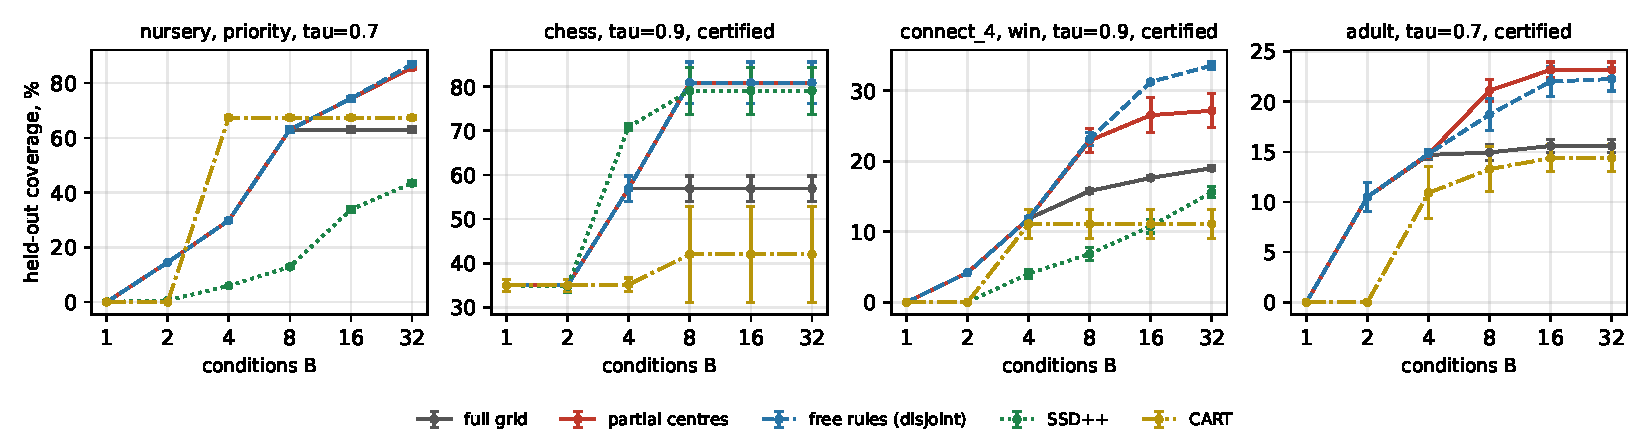
\includegraphics[width=\linewidth]{fig_coverage_budget}
\caption{Покрытие на отложенных строках в зависимости от бюджета условий на четырёх таблицах (среднее $\pm$ стандартная ошибка Надо--Бенжио по разбиениям). Частичные центры следуют за свободными непересекающимися правилами там, где полная сетка останавливается; \texttt{connect\_4}~--- таблица, на которой одна схема не может вместить то, что предлагают сорок два столбца. (Надписи на самом рисунке оставлены на английском.)}\label{fig:budget}
\end{figure}

Таблица~\ref{tab:counts} даёт подсчёты по 21 конфигурации с наблюдаемой чистотой и 10 сертифицированным, которые информативны (какой-либо метод выше 1\,\% покрытия на отложенных строках); рис.~\ref{fig:budget} показывает четыре из них в зависимости от бюджета. После поправки Холма частичные центры проигрывают непересекающимся правилам 16 из 109 ячеек с наблюдаемой чистотой и 3 из 53 сертифицированных и никогда не проигрывают полной сетке (39 и 15 побед сохраняются); описательные отметки дают ту же картину с бо́льшим числом отметок: по правилу наблюдаемой чистоты полная сетка проигрывает свободным непересекающимся правилам в 45 из 109 ячеек и выигрывает 2; с частичными центрами то же семейство схем проигрывает 21 и выигрывает 5 и закрывает медианно 85\,\% разрыва. Под сертификатом полная сетка проигрывает 20 из 53 ячеек; частичные центры проигрывают 6 (пять на \texttt{connect\_4}, раздел~\ref{sec:ssdpp}, и \texttt{nursery} при $\tau=0{,}7$, $B=32$: 61 против 67 пунктов) и выигрывают 2. При единственном бюджете $B=32$, по одной ячейке на конфигурацию (таблицы~\ref{tab:purity32} и~\ref{tab:cert32}): под сертификатом частичные центры идут вровень с непересекающимися правилами на 7 из 10 конфигураций и проигрывают на 3, а полную сетку превосходят на 6; по правилу наблюдаемой чистоты они выигрывают 2 из 21, идут вровень на 7 и проигрывают на 12, а полную сетку превосходят на 13. Поражения по правилу наблюдаемой чистоты приходятся на $B\ge16$ (20 из 21) на таблицах с наибольшим запасом столбцов (\texttt{connect\_4}, \texttt{mlc\_churn}, \texttt{credit}, \texttt{attrition}, \texttt{resume}, \texttt{wa\_churn}: таблица~\ref{tab:purity32}), где свободные правила продолжают добавлять непересекающиеся фрагменты из других столбцов после того, как четыре столбца схемы исчерпаны; под сертификатом эти фрагменты не проходят порог, и поражения исчезают. \texttt{car} входит в подсчёты с наблюдаемой чистотой (его разбиение, слитое внутри фолда, одинаково дорого обходится сетке и частичным центрам, раздел~\ref{sec:ablation}) и исключена из сертифицированных подсчётов как неинформативная; ни одно ключевое число от неё не зависит.

На невыровненном дизайне полная сетка покрывает 0,375 при любом бюджете (одно правило; второму нужно девять ячеек по 4 условия), тогда как частичные центры достигают 0,718 при $B=16$, наравне со свободными правилами; на выровненном дизайне полная сетка всё равно проигрывает (0,504 против 0,544), поскольку внедрённая 2-ячейка стоит девяти полных ячеек. При $B=32$ полная сетка в среднем тратит 7 условий: одна сетка содержит мало чистых полностью заданных ячеек. Это механизм рис.~\ref{fig:mech}: цена выравнивания~--- это цена фиксации каждой оси.

\subsection{Компактность описания}\label{sec:compact}
\begin{table}[t]\centering\small
\caption{Компактность при $B=32$ по информативным конфигурациям, на которых запускались все методы (\texttt{experiments/compactness.py}). Покрытие и потраченные условия~--- средние на отложенных строках по всем разбиениям; группы и различные столбцы, названные описанием, считаются на первом разбиении, поскольку набор столбцов не записывается по разбиениям. Дерево и SSD++ не записывают метки столбцов.}\label{tab:compact}
\begin{tabular}{llrrrrr}
\toprule
отбор & метод & ячейки & покрытие & условия & группы & столбцы\\
\midrule
чистота & полная сетка & 21 & 0{,}41 & 17{,}3 & 5{,}1 & 3{,}0\\
чистота & частичные центры & 21 & 0{,}46 & 16{,}4 & 5{,}5 & 3{,}9\\
чистота & жадная цепочка & 21 & 0{,}35 & 13{,}5 & 4{,}6 & 2{,}6\\
чистота & правила$_{\mathrm{непер}}$ & 21 & 0{,}49 & 22{,}3 & 7{,}6 & 8{,}3\\
чистота & правила (пересек.) & 21 & 0{,}59 & 26{,}6 & 10{,}1 & 10{,}2\\
чистота & дерево & 21 & 0{,}37 & 7{,}7 & 2{,}7 & --\\
чистота & SSD++ & 21 & 0{,}39 & 14{,}8 & 5{,}2 & --\\
\midrule
сертиф. & полная сетка & 10 & 0{,}33 & 7{,}7 & 2{,}9 & 2{,}6\\
сертиф. & частичные центры & 10 & 0{,}40 & 8{,}8 & 3{,}5 & 3{,}3\\
сертиф. & жадная цепочка & 10 & 0{,}30 & 6{,}8 & 3{,}0 & 2{,}2\\
сертиф. & правила$_{\mathrm{непер}}$ & 10 & 0{,}42 & 11{,}7 & 4{,}0 & 4{,}4\\
сертиф. & правила (пересек.) & 10 & 0{,}48 & 18{,}5 & 6{,}7 & 7{,}1\\
сертиф. & дерево & 10 & 0{,}34 & 3{,}9 & 1{,}4 & --\\
сертиф. & SSD++ & 10 & 0{,}32 & 14{,}8 & 4{,}5 & --\\
\bottomrule
\end{tabular}

\end{table}

Бюджет условий ограничивает длину описания; таблица~\ref{tab:compact} показывает, сколько методы фактически тратят при $B=32$ и сколько столбцов приходится держать в голове читателю. По правилу наблюдаемой чистоты частичные центры достигают 94\,\% покрытия свободных непересекающихся правил ($0{,}46$ против $0{,}49$) при 74\,\% условий ($16{,}4$ против $22{,}3$) и менее чем половине столбцов ($3{,}9$ против $8{,}3$); пересекающиеся правила достигают $0{,}59$, называя десять столбцов и тратя $27$ условий на группы, объединение которых не удерживает $\tau$ (таблица~\ref{tab:counts}). Под сертификатом направление то же, а разница в столбцах меньше~--- три четверти, а не меньше половины ($0{,}40$ против $0{,}42$ покрытия, $8{,}8$ против $11{,}7$ условий, $3{,}3$ против $4{,}4$ столбцов). Полная сетка и деревья (раздел~\ref{sec:treeopt}) ещё компактнее; полная сетка и CART платят за это покрытием, оптимальное дерево~--- нет; жадная цепочка компактна, потому что останавливается рано. Число столбцов у метода на сетках ограничено четырьмя по построению; у свободных правил оно растёт с бюджетом, поскольку каждый следующий непересекающийся фрагмент может прийти из нового столбца. Это вместе с непересекаемостью~--- то, что ограничение одной сеткой даёт по сравнению со свободными правилами; сертификат у них общий (раздел~\ref{sec:protocol}). \todo{Ещё не посчитано: число различных схем, на которых лежат свободные непересекающиеся правила при $B=32$ под сертификатом с $m=20$, и доля их покрытия, которую вмещает одна лучшая схема.}

\subsection{Под сертификатом}\label{sec:certified}
Таблица~\ref{tab:cert32}. Из 19 сертифицированных конфигураций на реальных таблицах 10 сертифицируют хоть что-то; девять, которые не сертифицируют ничего,~--- это три клинические таблицы ($N\le700$), \texttt{car}, \texttt{credit}, \texttt{resume}, \texttt{wa\_churn}, \texttt{attrition} и \texttt{splice}, где ни одна ячейка не достигает $n_{\min}$ при своём $\tau$ (раздел~\ref{sec:certificate}). Из шести внедрённых дизайнов три при $N=2\,000$ не сертифицируют почти ничего (\emph{xor}~--- 7,5\,\%, два других~--- 0), а три при $N=20\,000$ сертифицируют 90--96\,\% положительных строк. Парные подсчёты ниже~--- по десяти информативным реальным конфигурациям (53 ячейки). Главный результат здесь~--- ничья, и читать его следует именно так: одна схема с частичными центрами идёт вровень со свободными непересекающимися правилами в 45 из 53 ячеек, выигрывает 2 (\texttt{mushroom} при $B\le4$) и проигрывает 6 (\texttt{connect\_4} и \texttt{nursery} при $\tau=0{,}7$, $B=32$); против полной сетки она никогда не хуже и лучше в 18 из 53 ячеек. Ничья~--- ожидаемый результат, поскольку оба метода сертифицируют из одного семейства; при равном сертифицированном покрытии различается описание (раздел~\ref{sec:compact}). Независимая реимплементация трёх семейств кандидатов без пакета \texttt{vsf} (\texttt{experiments/partial\_centres\_external.py}: без правила ёмкости, без слияния уровней, фолды $5\times3$), запущенная на восьми таблицах до того, как большинство из них вошло в исследование, дала ту же картину (77 ничьих, 2 победы, 0 поражений по 79 ячейкам). Чистота объединения на отложенных строках достигает $\tau$ в 97\,\% разбиений для каждого метода под сертификатом против 60\,\% для пересекающихся правил по правилу наблюдаемой чистоты (таблица~\ref{tab:counts}). 97\,\%~--- среднее по конфигурациям: при $B=32$ частичные центры достигают $\tau$ в каждом разбиении на девяти из десяти и в 76\,\% разбиений на \texttt{mlc\_churn} (таблица~\ref{tab:split}). Доля на отложенных строках~--- это проверка, а не тест теоремы~\ref{thm:cert}: теорема ограничивает среднюю условную вероятность \emph{обучающих} строк сертифицированной ячейки, а чистота той же ячейки на отложенном фолде~--- зашумлённая оценка близкой величины, так что ячейка, средняя вероятность которой чуть выше $\tau$, падает ниже $\tau$ на отложенном фолде примерно в половине случаев, хотя ни один сертификат не ложен.

\subsection{Чистое покрытие и стабильность}\label{sec:net}

Одно лишь покрытие вознаграждает метод, добавляющий фрагменты, чистота которых не подтверждается, поэтому таблица~\ref{tab:net32} (приложение~\ref{app:tables}) ставит рядом покрытие и чистое покрытие (раздел~\ref{sec:method}, вычисленное на объединении на отложенных строках) для каждой конфигурации. Порядок различается между двумя правилами отбора. Под сертификатом среднее чистое покрытие по информативным ячейкам равно $0{,}23$ для частичных центров, $0{,}23$ для полной сетки, $0{,}22$ для непересекающихся и для пересекающихся правил и $0{,}18$ для дерева (SSD++ и оптимальное дерево впереди всех них; разделы~\ref{sec:treeopt} и~\ref{sec:ssdpp}). По правилу наблюдаемой чистоты оно равно $0{,}16$ для полной сетки и для частичных центров, $0{,}13$ для непересекающихся правил и дерева и $0{,}05$ для пересекающихся правил; по чистому покрытию частичные центры превосходят пересекающиеся правила в 44 из 109 ячеек и проигрывают 2: чем свободнее описание, тем бо́льшая часть его покрытия на обучении~--- фрагменты, не переживающие отложенный фолд (\texttt{titanic}, $\tau=0{,}7$: пересекающиеся правила $-0{,}24$, непересекающиеся $0{,}07$, частичные центры $0{,}08$, полная сетка $0{,}15$). При $m=20$ три непересекающихся метода на каждой таблице отличаются друг от друга на несколько пунктов. Урок~--- это эффект дисциплины отбора, а не эффект сетки: ячейки полной сетки велики, потому что их мало, а порог размера даёт более свободным методам ту же защиту.

Стабильность описания (среднее попарное сходство Жаккара выбранных строк по разбиениям) методы не различает: медианы $0{,}82$--$0{,}92$ по обоим правилам, выше всего у дерева ($0{,}90$--$0{,}92$), ниже всего у частичных центров и непересекающихся правил ($0{,}82$--$0{,}87$). Более свободное описание выбирается из большего числа кандидатов и сильнее меняется от выборки к выборке; разница мала.

\subsection{Деревья и жадные цепочки}\label{sec:trees}
Дерево CART глубины $\le4$ с $\min\_samples\_leaf=m$, лучшее по критерию и весу класса для каждого бюджета,~--- естественный конкурент, который тоже называет не более четырёх столбцов на лист и разбивает строки. По правилу наблюдаемой чистоты частичные центры превосходят его (парное $|t|\ge2$) в 39 из 109 ячеек и проигрывают 10 (при $B=32$: 9 побед, 12 ничьих, ни одного поражения); под сертификатом~--- 22 / 17 / 14 (при $B=32$: 5 / 3 / 2), но фильтр дерева не является сертификатом: его листья выращены по целевой переменной, а не взяты из семейства, фиксированного до её чтения, поэтому его 51,7 против 34,2 на \texttt{titanic} при $\tau=0{,}7$ не несут гарантии: чистота его объединения на отложенных строках там $0{,}89$ против $0{,}95$ у сертифицированной сетки~--- фильтр пропустил листья, которые сертификат по фиксированному семейству не пропустил бы. На дизайне с внедрённой сеткой CART жаден в корне и покрывает 2--4\,\% (\texttt{experiments/compare\_baselines.py --synthetic grid}). В разделе~\ref{sec:treeopt} запускается оптимальное дерево.

Жадная цепочка схем $S_1\subset S_2\subset S_3\subset S_4$ (добавлять столбец, больше всего улучшающий ключ ранжирования) хуже исчерпывающего победителя в 33 из 109 ячеек по правилу наблюдаемой чистоты и в 9 из 53 под сертификатом и никогда не лучше (средний разрыв при $B=32$: 6,3 и 3,4 пункта); на \texttt{chess} она так и не уходит от одномерного победителя (35\,\% против 84\,\% и 57\,\% у исчерпывающего поиска). Это и есть случай синергии, ради которого существует исчерпывающий поиск.

\subsection{Оптимальные деревья}\label{sec:treeopt}

Оптимальное дерево~--- сильнейший конкурент среди одиночных разбиений в исследовании, и итог таков: сравнимое покрытие, меньшее чистое покрытие у частичных центров (таблица~\ref{tab:treeopt}, приложение~\ref{app:tables}). По покрытию на отложенных строках по правилу наблюдаемой чистоты частичные центры превосходят его в 33 из 109 ячеек и проигрывают 13 (при $B=32$: $0{,}46$ против $0{,}43$ среднего покрытия); под сертификатом выигрывают 14 и проигрывают 15 ($0{,}40$ против $0{,}40$). По чистому покрытию оптимальное дерево явно впереди по обоим правилам ($0{,}20$ против $0{,}14$ и $0{,}33$ против $0{,}28$ при $B=32$): оно оптимизирует ровно эту величину, а его листья немногочисленны и велики. Там, где оно проигрывает в покрытии, оно проигрывает по той же причине, что и CART,~--- одно разбиение строк: на \texttt{attrition}, \texttt{credit} и \texttt{wa\_churn} частичные центры покрывают на $5$--$12$ пунктов больше, на \texttt{chess} и \texttt{mlc\_churn} дерево покрывает на $4$--$13$ больше. Две оговорки не позволяют считать это последним словом. Листья дерева выращены по целевой переменной, так что по сертифицированному правилу порог~--- фильтр, а не сертификат, в точности как для CART. И на \texttt{connect\_4} подгонка глубины~4 достигла десятиминутного лимита на $40$--$100\,\%$ разбиений (таблица~\ref{tab:treeopt}), так что приведённое там дерево~--- лучшее дерево DL8.5 к моменту лимита, а не доказанный оптимум; на всех остальных таблицах каждая подгонка завершилась. Сравнение решает более узкий вопрос, который стоит сформулировать: числа для CART из раздела~\ref{sec:trees}~--- не артефакт жадного дерева. По сравнению с CART, настроенным на покрытие, оптимальное взвешенное дерево при $B=32$ покрывает больше на девяти таблицах и меньше на шести; оптимальность покупает чистое покрытие, а не покрытие.

\subsection{Списки WRAcc}\label{sec:wracc}
Список, ранжированный по WRAcc,~--- это то, что возвращает инструмент поиска подгрупп, а порог чистоты~--- то, что добавляет к нему наша задача. С порогом список~--- это семейство свободных правил в другом порядке, и этот порядок стоит покрытия по сравнению с бюджетным максимальным покрытием по тем же правилам ($0{,}46$ против $0{,}59$ при $B=32$ по правилу наблюдаемой чистоты), зато выигрывает в чистоте на отложенных строках (объединение достигает $\tau$ в $71\,\%$ разбиений против $60\,\%$ при максимальном покрытии): верх ранжирования WRAcc~--- это крупные чистые правила. Против частичных центров это почти ничья по покрытию ($0{,}46$ против $0{,}46$; частичные центры выигрывают 27 из 109 ячеек и проигрывают 7, под сертификатом 10 и 1) при более низкой чистоте на отложенных строках ($71$ против $79\,\%$ разбиений). Без порога список вообще не является решением задачи: он покрывает гораздо больше ($0{,}83$ при $B=32$, превосходя частичные центры в 85 из 109 ячеек) при объединении, достигающем $\tau$ в $16\,\%$ разбиений, а на 18 из 21 конфигурации при $B=32$~--- ни в одном (\texttt{sex = female} первым на \texttt{titanic}, чистота $0{,}73$, затем правила, добавляющие строки быстрее, чем положительные). Именно порог чистоты, а не поиск, отделяет описание того, где находится целевая переменная, от ранжирования того, где она перепредставлена; инструмент «из коробки» отвечает на второй вопрос.

\subsection{SSD++}\label{sec:ssdpp}
SSD++ оптимизирует сжатие всего столбца целевой переменной, а не покрытие при пороге чистоты, и сравнение показывает обе стороны этого. По покрытию на отложенных строках при $\tau$ частичные центры превосходят его в 63 из 109 ячеек с наблюдаемой чистотой и проигрывают 16 (сертифицированно: 34 / 16 / 3); при $B=32$ его среднее покрытие $0{,}39$ против $0{,}46$ (сертифицированно $0{,}32$ против $0{,}40$). По чистоте на отложенных строках он лучший среди методов, запущенных на каждой таблице: $0{,}96$ под сертификатом и $0{,}83$ по правилу наблюдаемой чистоты против $0{,}91$ и $0{,}76$ у частичных центров, и среди этих методов его чистое покрытие при $B=32$ наибольшее по обоим правилам ($0{,}31$ и $0{,}26$ против $0{,}28$ и $0{,}14$ у частичных центров); оптимальное дерево на своих ячейках ещё выше (раздел~\ref{sec:treeopt}). Эти два факта~--- один и тот же факт, и таблица~\ref{tab:net32} показывает их по конфигурациям: список правил перестаёт добавлять правила, когда они больше не окупаются в длине кода, так что возвращаемое им мало и чисто; цель покрытия продолжает добавлять группы ровно на уровне $\tau$, и каждая такая группа снижает чистую оценку. Мы не утверждаем, что частичные центры превосходят SSD++; по цели, которую оптимизирует SSD++, это не так. Задача статьи фиксирует цель~--- покрытие при пороге чистоты,~--- и по этой цели одна сетка с частичными центрами впереди; читателю, чей вопрос~--- «самое чистое небольшое описание», следует предпочесть список правил. Для сравнения важно ещё одно свойство списка: его $i$-е правило применяется к остатку после первых $i-1$, включая правила для \emph{другого} класса, поэтому более позднее правило может быть чистым на остатке там, где ни одна конъюнкция не чиста на таблице. На \texttt{splice} ($\tau=0{,}9$, $m=20$) конъюнктивное семейство длины $\le3$ пусто на 9 из 15 обучающих фолдов, каждый метод на сетках и правилах покрывает $4$--$5\,\%$ при $B=32$ с чистотой объединения на отложенных строках $0{,}61$, а SSD++ покрывает $19\,\%$ при чистоте на отложенных строках $0{,}83$, ниже $\tau$. Упорядоченная семантика «иначе»~--- самостоятельный язык описаний; частичные центры могли бы её перенять (пластина минус более ранний стержень~--- всё ещё область того же куба), и мы оставляем это на будущее.

\paragraph{Где сетка всё ещё дорога: \texttt{connect\_4}.} Пять из шести сертифицированных поражений от непересекающихся правил~--- на \texttt{connect\_4} ($67\,557\times42$, три значения на клетку; шестое~--- \texttt{nursery} при $B=32$, раздел~\ref{sec:mechanism}): для целевого значения \texttt{win} при $\tau=0{,}9$, $B=32$ частичные центры покрывают $27\,\%$ против $34\,\%$ у непересекающихся правил ($43\,\%$ у пересекающихся); для целевого значения \texttt{loss} при $\tau=0{,}7$~--- $6\,\%$ против $12\,\%$. Свободные правила выбирают свои четыре столбца для каждого правила, и сорок два столбца дают им много чистых конъюнкций из четырёх клеток на разных позициях доски; одна схема не может их вместить. Это тот случай, в котором ограничение одной сеткой должно было проиграть, и оно проигрывает; на \texttt{chess} ($M=36$) частичные центры и непересекающиеся правила идут вровень на $81\,\%$ там, где у полной сетки $57\,\%$.

\subsection{Сколько столбцов нужно семейству}\label{sec:maxd}
Предел $|S|\le4$ задан отображением; теорема~\ref{thm:cert} от него не зависит. Сертификат верен для любой максимальной размерности $D$, зафиксированной до чтения целевой переменной, и $D$ действует на него дважды: бо́льшее $D$ добавляет ячейки-кандидаты и увеличивает $T$, что поднимает порог для каждой ячейки. Таблица~\ref{tab:maxd} измеряет итоговый эффект. Для $D=2,3,4$ семейство пересчитывается (различные множества строк неслитых ячеек не более чем по $D$ столбцам; на \texttt{titanic} $T=2\,943$ при $D=4$ против $3\,102$ в продукте, где учитываются и слитые разбиения), а покрытие~--- доля положительных строк в объединении всех сертифицированных ячеек на всех строках при $\alpha=0{,}05$ и собственных $\tau$ и $m$ каждой конфигурации. Это верхняя граница для любого отбора: бюджета нет, отложенного фолда нет. Правило зафиксировано коммитом до запуска.

\begin{table}[t]\centering\small
\caption{Сертифицированное покрытие (\%) на всех строках, когда семейство ограничено ячейками не более чем по $D$ столбцам, с $T$, пересчитанным для каждого $D$: объединение всех сертифицированных ячеек, без бюджета и без отложенного фолда. Конфигурации с непустым сертификатом; \texttt{connect\_4} не посчитан. \todo{скрипт, порождающий таблицу, и проверка в \texttt{check\_numbers.py}}}\label{tab:maxd}
\begin{tabular}{lrrrr}
\toprule
конфигурация & $D\le2$ & $D\le3$ & $D\le4$ & четвёртый столбец\\
\midrule
titanic ($\tau=0{,}7$) & 47{,}7 & 47{,}4 & 47{,}4 & 0\\
chess\_krkp & 35{,}0 & 94{,}2 & 94{,}2 & 0\\
mushroom & 100 & 100 & 100 & 0\\
hmda & 15{,}4 & 15{,}4 & 15{,}4 & 0\\
mlc\_churn & 12{,}9 & 12{,}9 & 12{,}9 & 0\\
adult & 34{,}3 & 49{,}2 & 51{,}8 & $+2{,}6$\\
nursery (spec\_prior) & 21{,}1 & 56{,}0 & 60{,}5 & $+4{,}5$\\
nursery (priority) & 63{,}0 & 69{,}8 & 82{,}4 & $+12{,}6$\\
\bottomrule
\end{tabular}
\end{table}

В пяти из восьми конфигураций покрытие перестаёт расти при $D\le3$ (\texttt{titanic}, \texttt{chess}, \texttt{mushroom}, \texttt{hmda}, \texttt{mlc\_churn}); в трёх из них (\texttt{mushroom}, \texttt{hmda}, \texttt{mlc\_churn}) оно насыщается уже при $D=2$, так что о четвёртом столбце как таковом они говорят мало. На \texttt{titanic} семейство из двух столбцов сертифицирует чуть больше, чем из четырёх (47,7 против 47,4\,\%): рост $T$ стоит больше, чем добавляют лишние ячейки. Четвёртый столбец добавляет в трёх конфигурациях: \texttt{adult} ($+2{,}6$ пункта) и оба целевых значения \texttt{nursery} ($+4{,}5$ и $+12{,}6$), из них наблюдательная только \texttt{adult}. Конфигурации, где сертификат пуст при $D=4$, пусты и при $D=2$ и $D=3$: меньшее семейство не расширяет охват сертификата. Полезная размерность растёт с размером таблицы, а не равна четырём; четыре~--- предел отображения, и таблица~\ref{tab:maxd}~--- его цена там, где она измерена. \todo{Ещё не посчитано: $D=5$ на всех таблицах, где перебор посилен (правило по вычислительной стоимости, а не по результату); \texttt{connect\_4} при $D\le3$; то же сравнение под бюджетом на отложенных строках.}

\subsection{Сертифицированное покрытие как функция порога}\label{sec:taucurve}
Поскольку гарантия теоремы~\ref{thm:cert} одновременна по $\tau$, сертифицированное покрытие~--- не число при одном вручную выбранном пороге, а кривая, которую можно прочитать целиком и выбрать по ней порог после просмотра данных. Кривая заменяет подсчёт «непуст на 10 из 19 конфигураций при порогах раздела~\ref{sec:protocol}» порогом, при котором сертификат каждой конфигурации становится пустым. Её цена измеряется против редукции Тароне, вычисленной при нижнем пороге $\tau_0$, зафиксированном без целевой переменной и корректной для всех $\tau\ge\tau_0$ (раздел~\ref{sec:certificate}): разрыв между двумя кривыми~--- это цена права сдвигать порог ниже $\tau_0$. \todo{Рисунок и числа ещё не посчитаны: сертифицированное покрытие на всех строках в зависимости от $\tau$ для каждой конфигурации, семейная оценка против Тароне при $\tau_0$ (значение фиксируется до запуска, без целевой переменной); чистота сертифицированного объединения на отложенных строках как проверка, а не тест, как в разделе~\ref{sec:certified}.}

\subsection{Абляции: правило ёмкости и порог размера}\label{sec:ablation}
\texttt{experiments/ablations.py} варьирует делитель ёмкости ($N_{\mathrm{train}}/5$, $/10$, $/20$, без слияния) и порог размера $m\in\{1,5,20\}$ на восьми таблицах при $B=32$. Правило ёмкости инертно на семи из них: выигрывающие схемы никогда не достигают потолка, и покрытие меняется не более чем на $0{,}1$ пункта. На \texttt{car\_evaluation}~--- полном факторном плане из $1\,728$ строк на потолке~--- любое изменение теряет покрытие: $-7{,}1$ пункта при более мягком правиле ($N/5$) или без него, $-8{,}6$ при более жёстком ($N/20$),~--- для полной сетки и для частичных центров одинаково: слитые уровни объединяют разреженные ячейки выше порога, а дальнейшее слияние разделяет целевую переменную. Поэтому правило~--- не настроечный рычаг в пользу метода; это ограничение отображения, которое ничего не стоит на большинстве таблиц и несколько пунктов~--- на одной.

Порог размера~--- рычаг, который имеет значение, и сильнее всего он действует на более свободные описания. При переходе от $m=1$ к $m=20$ непересекающиеся правила теряют $4{,}6$ пункта покрытия и повышают долю разбиений, чистота которых на отложенных строках достигает $\tau$, с $77$ до $91\,\%$; частичные центры теряют $3{,}7$ пункта ($85\to87\,\%$); полная сетка теряет $3{,}0$ ($94\to83\,\%$: её ячейки и так велики, и порог убирает немногие мелкие чистые, которые у неё были). Потраченные условия при $B=32$ падают с $29$ до $14$ у правил и с $25$ до $13$ у частичных центров. Раздел~\ref{sec:net}~--- тот же эффект, увиденный через чистое покрытие.

\subsection{Фиксированная сетка порогов}\label{sec:grid}
Пороги из раздела~\ref{sec:protocol} заданы вручную, поэтому сравнение по наблюдаемой чистоте было повторено на одной сетке для каждой таблицы: каждая из 19 пар (таблица, целевое значение) при $\tau\in\{0{,}7;\ 0{,}9\}$ и $m\in\{1,20\}$, с фолдами, повторами и наибольшим $d$ своей конфигурации, для полной сетки, частичных центров, жадной цепочки, трёх базовых методов на правилах и CART (\texttt{compare\_baselines.py --config-set grid}): 76 конфигураций, из которых 73 информативны, 373 ячейки. Таблица~\ref{tab:grid} даёт результат по порогам при $B=32$.

\begin{table}[t]\centering\small\setlength{\tabcolsep}{3.5pt}
\caption{Сравнение по наблюдаемой чистоте на одной фиксированной сетке порогов, $B=32$: число информативных конфигураций $n$; отметки ($|t|\ge2$) частичных центров (част.) и полной сетки против свободных непересекающихся правил (прав.); средние по конфигурациям покрытия и чистого покрытия на отложенных строках в пунктах и доли разбиений, в которых объединение на отложенных строках достигает $\tau$, для полной сетки, частичных центров и непересекающихся правил. Получено \texttt{experiments/paper\_tables.py} из \texttt{pairwise\_grid.csv}.}\label{tab:grid}
\begin{tabular}{rrr rrr rrr rrr rrr rrr}
\toprule
& & & \multicolumn{3}{c}{част.\ vs прав.} & \multicolumn{3}{c}{сетка vs прав.} & \multicolumn{3}{c}{покрытие} & \multicolumn{3}{c}{чистое покрытие} & \multicolumn{3}{c}{разбиения с $\ge\tau$, \%}\\
\cmidrule(lr){4-6}\cmidrule(lr){7-9}\cmidrule(lr){10-12}\cmidrule(lr){13-15}\cmidrule(lr){16-18}
$\tau$ & $m$ & $n$ & $+$ & $=$ & $-$ & $+$ & $=$ & $-$ & сетка & част. & прав. & сетка & част. & прав. & сетка & част. & прав.\\
\midrule
0{,}7 & 1 & 19 & 3 & 6 & 10 & 0 & 7 & 12 & $49$ & $55$ & $57$ & $22$ & $18$ & $9$ & $79$ & $74$ & $67$\\
0{,}7 & 20 & 18 & 4 & 9 & 5 & 3 & 7 & 8 & $49$ & $55$ & $55$ & $23$ & $23$ & $18$ & $86$ & $83$ & $82$\\
0{,}9 & 1 & 19 & 2 & 5 & 12 & 1 & 4 & 14 & $32$ & $35$ & $37$ & $8$ & $0$ & $-15$ & $60$ & $55$ & $46$\\
0{,}9 & 20 & 17 & 2 & 8 & 7 & 1 & 6 & 10 & $32$ & $34$ & $34$ & $20$ & $19$ & $19$ & $67$ & $67$ & $63$\\
\midrule
\multicolumn{2}{l}{все} & 73 & 11 & 28 & 34 & 5 & 24 & 44 & $41$ & $45$ & $46$ & $18$ & $15$ & $7$ & $73$ & $70$ & $64$\\
\bottomrule
\end{tabular}

\end{table}

Подсчёты из раздела~\ref{sec:mechanism} не зависят от выбранных нами порогов. На сетке частичные центры проигрывают свободным непересекающимся правилам в 62 из 373 ячеек и выигрывают 39 (45 и 25 после поправки Холма); при $B=32$ они проигрывают на 34 из 73 конфигураций и выигрывают на 11. Полная сетка проигрывает 133 ячейки и выигрывает 17, а частичные центры лучше полной сетки в 109 ячейках и никогда не хуже. Порог размера делает на сетке то же, что раздел~\ref{sec:ablation} обнаружил на восьми таблицах: при $B=32$ частичные центры проигрывают на 22 из 38 конфигураций с $m=1$ и на 12 из 35 с $m=20$, а при $\tau=0{,}9$ среднее чистое покрытие растёт с $8$, $0$ и $-15$ пунктов (полная сетка, частичные центры, непересекающиеся правила) при $m=1$ до $20$, $19$ и $19$ при $m=20$. Порог $\tau=0{,}9$ при $m=1$~--- тот, на котором ни один метод не выполняет обещания: объединение на отложенных строках достигает $\tau$ в $60$, $55$ и $46\,\%$ разбиений. Поражения приходятся на одни и те же таблицы при любом пороге (\texttt{connect\_4} с целевым значением \texttt{loss}, \texttt{mlc\_churn} и \texttt{wa\_churn} проигрывают при всех четырёх), а победы не являются свидетельством в пользу сетки: частичные центры впереди при всех четырёх порогах только на \texttt{breast\_cancer\_wisconsin}~--- таблице, на которой жадная упаковка свободных правил дальше всего от точного оптимума (раздел~\ref{sec:packing}). Те же пороги прогнаны и при сертифицированном отборе (\texttt{run\_jobs.py --plan grid\_certified}): каждая пара (таблица, целевое значение) при $\tau\in\{0{,}7;\ 0{,}9\}$ со своим порогом размера $m$, который везде меньше наименьшей сертифицируемой ячейки и поэтому не является измерением этой сетки; 38 конфигураций, из которых 18 информативны, 94 ячейки (таблица~\ref{tab:gridcert}). Сертифицированные подсчёты тоже не зависят от порогов. Частичные центры идут вровень со свободными непересекающимися правилами в 76 из 94 ячеек, выигрывают 11 и проигрывают 7 (6, 84 и 4 после поправки Холма); при $B=32$ они идут вровень на 13 из 18 конфигураций, выигрывают на 1 и проигрывают на 4. Поражения~--- те же, что в разделе~\ref{sec:mechanism}: \texttt{connect\_4} (шесть ячеек) и \texttt{nursery} с целевым значением \texttt{priority} при $\tau=0{,}7$, $B=32$. Победы~--- на \texttt{breast\_cancer\_wisconsin}, \texttt{mushroom}, \texttt{nursery} и \texttt{connect\_4} при малых бюджетах; как и на сетке с наблюдаемой чистотой, победы на \texttt{breast\_cancer\_wisconsin} приходятся на таблицу, где жадная упаковка свободных правил дальше всего от оптимума. Полная сетка проигрывает свободным непересекающимся правилам 33 ячейки, а частичные центры никогда не хуже неё. Объединение на отложенных строках достигает $\tau$ в 98\,\% разбиений у трёх непересекающихся методов. При $\tau=0{,}7$ сертификат непуст на 12 из 19 пар, среди них три наблюдательные таблицы, пустые при порогах исследования: \texttt{thyroid\_recurrence}, \texttt{breast\_cancer\_wisconsin} и \texttt{splice} (объединение которой достигает $\tau$ в 87\,\% разбиений). На сетке не повторялись и потому по-прежнему зависят от порогов из раздела~\ref{sec:protocol}: сравнения с оптимальным деревом, SSD++ и списками WRAcc, которые сертифицированный прогон на сетке покрывает лишь на половине информативных конфигураций.

\begin{table}[t]\centering\small\setlength{\tabcolsep}{3.5pt}
\caption{Сертифицированное сравнение на тех же порогах, $B=32$, каждая конфигурация со своим порогом размера $m$ («свой»); столбцы как в таблице~\ref{tab:grid}. Получено \texttt{experiments/paper\_tables.py} из \texttt{pairwise\_grid\_certified.csv}.}\label{tab:gridcert}
\begin{tabular}{rrr rrr rrr rrr rrr rrr}
\toprule
& & & \multicolumn{3}{c}{част.\ vs прав.} & \multicolumn{3}{c}{сетка vs прав.} & \multicolumn{3}{c}{покрытие} & \multicolumn{3}{c}{чистое покрытие} & \multicolumn{3}{c}{разбиения с $\ge\tau$, \%}\\
\cmidrule(lr){4-6}\cmidrule(lr){7-9}\cmidrule(lr){10-12}\cmidrule(lr){13-15}\cmidrule(lr){16-18}
$\tau$ & $m$ & $n$ & $+$ & $=$ & $-$ & $+$ & $=$ & $-$ & сетка & част. & прав. & сетка & част. & прав. & сетка & част. & прав.\\
\midrule
0{,}7 & свой & 12 & 1 & 8 & 3 & 0 & 6 & 6 & $48$ & $53$ & $53$ & $35$ & $35$ & $37$ & $97$ & $97$ & $97$\\
0{,}9 & свой & 6 & 0 & 5 & 1 & 0 & 2 & 4 & $42$ & $48$ & $49$ & $36$ & $37$ & $37$ & $100$ & $100$ & $100$\\
\midrule
\multicolumn{2}{l}{все} & 18 & 1 & 13 & 4 & 0 & 8 & 10 & $46$ & $51$ & $52$ & $35$ & $36$ & $37$ & $98$ & $98$ & $98$\\
\bottomrule
\end{tabular}

\end{table}

\subsection{Точная упаковка}\label{sec:packing}
Два отбора в протоколе эвристичны: непересекающаяся упаковка частичных центров внутри схемы, где схема выбирается по результату этой упаковки, и бюджетный жадный алгоритм по свободным непересекающимся правилам. \texttt{experiments/packing\_exact.py} решает оба как целочисленные программы~--- максимизировать число покрытых положительных строк при ограничении бюджета условий и не более чем одном выбранном кандидате на обучающую строку (HiGHS через \texttt{scipy})~--- над теми же кандидатами и теми же обучающими фолдами, для каждой схемы в частичном случае (схемы отсекаются по числу положительных строк в объединении их кандидатов, так что схема решается, только если может превзойти текущего лидера). Таблицы~--- восемь, на которых это посильно (\texttt{titanic}, три клинические таблицы, \texttt{car}, \texttt{nursery}, \texttt{hmda}): десять конфигураций с наблюдаемой чистотой и восемь сертифицированных, первые пять разбиений, шесть бюджетов, 540 ячеек; каждая программа достигла доказанной оптимальности, самая долгая~--- за 31 секунду. Под сертификатом жадный алгоритм в среднем отстаёт от точного оптимума на $0{,}01$ пункта для частичных центров (наибольший разрыв $1{,}4$, на \texttt{nursery}) и на $0{,}07$ для непересекающихся правил (наибольший $6{,}8$). По правилу наблюдаемой чистоты, где пулы содержат много мелких чистых на обучении ячеек, средний разрыв составляет $0{,}6$ пункта для частичных центров и $1{,}0$ для непересекающихся правил, с наибольшими разрывами ($12$ пунктов) на \texttt{breast\_cancer\_wisconsin} и \texttt{breast\_cancer} при $B=32$ и $m=1$. Отсюда два следствия. Жадный алгоритм стоит частичным центрам меньше, чем свободным правилам, так что точный разрыв между двумя методами немного больше приведённого ($0{,}7$ против $0{,}3$ пункта в среднем по этим ячейкам, $3{,}7$ против $3{,}1$ при $B=32$), а не меньше: оставшаяся цена одной сетки принадлежит сетке, а не упаковке. И точное решение посильно на таблицах такого размера, но не внутри поиска по всем схемам широкой таблицы; методом остаётся жадный алгоритм с этой оценкой его стоимости.

\subsection{Вычислительные затраты}
Время отбора на разбиение (среднее по бюджетам и правилам отбора, одно ядро): полная сетка 7,3\,с и частичные центры 8,4\,с на \texttt{adult} ($N=48\,842$, $M=12$); 5,9 / 9,8\,с на \texttt{chess} ($N=3\,196$, $M=36$, $58\,905$ схем размера~4; время однократного запуска на свободном ядре, поскольку перезапуск $5\times3$ выполнялся двенадцатью параллельными процессами); 2,2 / 9,6\,с на \texttt{mushroom}; меньше секунды на каждой таблице с $M\le 20$ и $N\le 8\,000$. Частичный поиск не перебирает новых ячеек; его дополнительная стоимость~--- непересекающаяся упаковка по пулу каждой схемы, которая растёт с числом подходящих подъячеек (у \texttt{mushroom} при $\tau=0{,}9$ их много). Свободные правила стоят столько же, сколько сетка, на каждой таблице; дерево быстрее всех. SSD++~--- выброс: на \texttt{adult} его подгонка занимала от 80\,с до 15\,ч на разбиение при сертифицированном отборе (медиана меньше двух минут), поскольку лучевой поиск MDL иногда доходил до предела в 40 правил; остальные методы различаются между разбиениями не более чем вдвое.

\section{Заключение}
Мы задали два вопроса о свободных конъюнктивных правилах не более чем из четырёх условий. Какие из них переживают поиск: те, чьё число положительных строк проходит порог по семейству различных множеств строк всех ячеек не более чем по четырём столбцам,~--- оценка объединения по семейству, фиксированному до чтения целевой переменной, с порогом, корректным для гетерогенных строк и одновременным по $\tau$. На чистом шуме он не сертифицирует ни одной ложной ячейки за 1\,000 запусков, тогда как посхемный сертификат делает это в 67\,\%; его цена логарифмична по числу столбцов и велика по чистоте; он пуст на таблицах из нескольких сотен строк и непуст на 10 из 19 реальных конфигураций при порогах исследования, три из которых наблюдательные; на тех же фолдах он превосходит контрольное разбиение~--- единственную альтернативу, применимую ко всем методам,~--- на четверть сертифицированного покрытия и по доле сертифицированных объединений, удерживающих $\tau$ на отложенных строках (97 против 49\,\%). У дерева или списка правил, подогнанного под целевую переменную, фиксированного семейства нет, и их можно сертифицировать только разбиением строк. Какая часть пережившего помещается в одну картинку: почти всё. Центры на части осей~--- свободные правила, ограниченные столбцами одной схемы,~--- идут вровень со свободными непересекающимися правилами в 45 из 53 сертифицированных ячеек при порогах исследования и в 76 из 94 на фиксированной сетке порогов; не помещается то, что лежит на других столбцах широких таблиц (\texttt{connect\_4}, где одна схема из четырёх столбцов не может вместить то, что предлагают сорок два), и один бюджет \texttt{nursery}, а по правилу наблюдаемой чистоты свободные правила всё ещё вмещают больше на таблицах с большим запасом столбцов. Потеря полной сетки происходит от фиксации каждой оси, а не от общих столбцов. Одна схема добавляет примерно при равном сертифицированном покрытии непересекаемость и описание, называющее меньше столбцов ($3{,}3$ против $4{,}4$ под сертификатом, $3{,}9$ против $8{,}3$ по правилу наблюдаемой чистоты). Против оптимального дерева глубины~4, подогнанного под ту же цель, частичные центры сравнимы по покрытию и отстают по чистому покрытию; читателю, которому сертификат не нужен, следует предпочесть дерево. Четыре столбца~--- предел отображения; на измеренных конфигурациях сертифицированное покрытие перестаёт расти на трёх в пяти из восьми, а четвёртый добавляет на \texttt{adult} и \texttt{nursery}. Сравнение также зафиксировало две вещи о том, как такие методы следует сравнивать: пересекающееся объединение правил, каждое из которых имеет чистоту $\tau$, не имеет чистоты $\tau$, а порог размера~--- то, что удерживает свободные описания честными на отложенных данных. Отсюда два направления. Упорядоченную семантику («иначе»), которая позволяет SSD++ находить чистые остатки на \texttt{splice}, где ни одна конъюнкция не чиста, можно дать частичным центрам, не выходя за пределы куба. А покупает ли общая картинка читаемость сверх измеренной компактности~--- вопрос о людях, а не о таблицах; здесь это не утверждается.

\section{Ограничения}
Отображение одной сеткой~--- то, откуда возникло ограничение, и общая картинка вполне может читаться легче, чем список правил; мы этого не измеряли, и ничто в статье на этом не основано. Инструмент описан (раздел~\ref{sec:display}), но не оценён: таблица~\ref{tab:properties} перечисляет, что содержит каждый вывод, а недостающее свидетельство~--- контролируемое исследование чтения в сравнении с деревом и списком правил; трёхмерное отображение вполне может читаться хуже дерева в простых задачах поиска значения. Показано, что ограничение покупает непересекаемость, фиксированное семейство и описание короче, чем у свободных правил (таблица~\ref{tab:compact}), но не короче, чем у дерева; стоят ли они того покрытия, которого ограничение всё ещё стоит на широких таблицах,~--- решать пользователю. Предел в четыре столбца задан отображением; раздел~\ref{sec:maxd} измеряет его цену на восьми конфигурациях на всех строках, а не под бюджетом на отложенных строках. Мощность сертификата при $N\le 500$ пренебрежимо мала; при $\tau=0{,}9$ он ничего не сертифицирует на \texttt{titanic}. Правило ёмкости $\lfloor N/10\rfloor$ взаимодействует с фолдами (\texttt{car}: полный факторный план на пороге ёмкости сливается внутри фолда, но не на всех строках, $+15$ пунктов кажущегося разрыва). Числовые столбцы разбиваются на интервалы до поиска; интервалы не оптимизируются. Семнадцать таблиц с $M\le 60$~--- это охват свидетельств; \texttt{splice} показывает, что при $\tau=0{,}9$ и $m=20$ конъюнктивное семейство длины $\le3$ пусто на большинстве обучающих фолдов, а \texttt{connect\_4}~--- что ограничение одной сеткой всё ещё стоит шести-семи пунктов там, где столбцов много и они похожи. Высокоразмерным таблицам нужен не зависящий от целевой переменной предварительный отбор признаков до фиксации семейства; мы его не строили. У \texttt{connect\_4} один повтор, поэтому её отметки опираются на четыре степени свободы (14 на \texttt{chess} и \texttt{splice}). Пороги чистоты заданы вручную для каждой конфигурации (раздел~\ref{sec:protocol}), а не одним правилом. Раздел~\ref{sec:grid} повторяет сравнение методов на сетках и на правилах на одной фиксированной сетке порогов при обоих правилах отбора и находит те же подсчёты; сравнения с оптимальным деревом, SSD++ и списками WRAcc там не повторялись, так что каждый подсчёт для них зависит от выбранных порогов. Гарантия сертификата даётся на каждое значение целевой переменной и направление и предполагает независимость при заданных столбцах, которую \texttt{titanic} нарушает. Упаковки жадные; раздел~\ref{sec:packing} оценивает, чего это стоит, только на малых таблицах.

\section{Воспроизводимость}
Код: \todo{Zenodo DOI}. Файл \texttt{PAPER.md} в репозитории перечисляет по порядку скрипт, порождающий каждую таблицу, рисунок и приведённое число; \texttt{requirements-experiments.txt} закрепляет версии всех пакетов, используемых в экспериментах (\texttt{experiments/setup\_experiments.py} устанавливает их, включая два, которым нужна пропатченная установка). Каждое число получено скриптом из \texttt{experiments/} с зерном 0 из данных, загруженных через манифест, и \texttt{experiments/check\_numbers.py} завершается с ошибкой, если число, приведённое в тексте, расходится с результатами. Каждая таблица в \texttt{benchmark\_data/} побайтно восстанавливается скриптом \texttt{experiments/build\_*.py} из закреплённого публичного источника (URL и SHA-256 источника и результата записаны в манифесте); поэтому предобработка каждой таблицы~--- перекодирование уровней, квантильные интервалы, сконструированные столбцы \texttt{titanic}~--- это код, а не описание. \texttt{titanic}~--- обучающий файл Kaggle, взятый из публичного зеркала, поскольку страница соревнования требует входа. Использование ИИ-помощника: части кода, скрипты экспериментов и черновик этого текста созданы с помощью ИИ-помощника для программирования (Claude, Anthropic) под руководством авторов; история репозитория фиксирует созданные им коммиты. Авторы проверили каждую строку кода и каждое приведённое здесь число и несут за них полную ответственность.


\appendix
\section{Таблицы по конфигурациям}\label{app:tables}
Три таблицы, которые обобщает текст разделов~\ref{sec:certificate}, \ref{sec:net} и~\ref{sec:treeopt}, по строке на конфигурацию.

\begin{table}[p]\centering\footnotesize\setlength{\tabcolsep}{3.5pt}
\caption{Семейный сертификат против разбиения на исследовательскую и контрольную части на тех же фолдах: покрытие на отложенных строках (пункты) при $B=32$ и, для частичных центров, доля разбиений ($\ge\tau$), в которых чистота объединения на отложенных строках достигает $\tau$. «--»: ни один метод не достигает $1\,\%$ покрытия на отложенных строках по этому правилу, так что конфигурация неинформативна и исключена из парного сравнения. У четырёх конфигураций, неинформативных по обоим правилам (\texttt{car}, \texttt{resume}, \texttt{breast\_cancer}, \texttt{splice}), строки нет. У набора данных, запущенного для двух целевых значений или двух порогов размера, целевое значение или $m$ указаны в скобках~--- здесь и во всех таблицах ниже. Получено \texttt{experiments/paper\_tables.py}.}\label{tab:split}
\begin{tabular}{llrrrrrrrrrr}
\toprule
& & \multicolumn{5}{c}{семейный сертификат} & \multicolumn{5}{c}{контрольное разбиение}\\
набор & $\tau$ & сетка & частичн. & прав.$_{\mathrm{непер}}$ & дерево & $\ge\tau$ & сетка & частичн. & прав.$_{\mathrm{непер}}$ & дерево & $\ge\tau$\\
\midrule
adult & 0{,}7 & 16 & 23 & 22 & 14 & 100 & 4 & 3 & 5 & 7 & 30\\
attrition & 0{,}5 & -- & -- & -- & -- & -- & 0 & 0 & 0 & 2 & 0\\
breast\_cancer\_wisconsin & 0{,}9 & -- & -- & -- & -- & -- & 0 & 4 & 4 & 1 & 8\\
chess\_krkp & 0{,}9 & 57 & 81 & 81 & 41 & 100 & 54 & 74 & 74 & 51 & 100\\
connect\_4 (loss) & 0{,}7 & 6 & 6 & 12 & 10 & 100 & 2 & 4 & 7 & 6 & 60\\
connect\_4 (win) & 0{,}9 & 19 & 27 & 34 & 11 & 100 & 21 & 22 & 23 & 9 & 100\\
credit & 0{,}7 & -- & -- & -- & -- & -- & 3 & 2 & 2 & 2 & 12\\
hmda & 0{,}5 & 15 & 15 & 15 & 15 & 100 & 1 & 6 & 6 & 7 & 44\\
mlc\_churn & 0{,}7 & 9 & 9 & 9 & 12 & 76 & 4 & 12 & 11 & 7 & 96\\
mushroom & 0{,}9 & 96 & 98 & 98 & 96 & 100 & 87 & 89 & 97 & 96 & 100\\
nursery (priority) & 0{,}7 & 40 & 61 & 67 & 67 & 100 & 54 & 58 & 57 & 49 & 100\\
nursery (spec\_prior) & 0{,}9 & 42 & 49 & 49 & 23 & 100 & 41 & 43 & 36 & 22 & 100\\
thyroid\_recurrence & 0{,}9 & -- & -- & -- & -- & -- & 0 & 0 & 3 & 0 & 0\\
titanic & 0{,}7 & 34 & 34 & 34 & 52 & 100 & 7 & 0 & 0 & 16 & 0\\
wa\_churn & 0{,}7 & -- & -- & -- & -- & -- & 3 & 1 & 1 & 5 & 8\\
\bottomrule
\end{tabular}

\end{table}

\begin{table}[p]\centering\scriptsize\setlength{\tabcolsep}{3pt}
\caption{Покрытие (пок.) и чистое покрытие (чист.) на отложенных строках, в пунктах, объединения выбранных групп при $B=32$ для каждой информативной конфигурации. Чистое покрытие $(k-\tfrac{\tau}{1-\tau}(n-k))/P$ отрицательно, когда объединение на отложенных строках ниже $\tau$. Получено \texttt{experiments/paper\_tables.py}.}\label{tab:net32}
\begin{tabular}{lllrrrrrrrrrrrr}
\toprule
& & & \multicolumn{2}{c}{частичн.} & \multicolumn{2}{c}{сетка} & \multicolumn{2}{c}{прав.$_{\mathrm{непер}}$} & \multicolumn{2}{c}{прав.} & \multicolumn{2}{c}{дерево} & \multicolumn{2}{c}{SSD++}\\
отбор & набор & $\tau$  & пок. & чист. & пок. & чист. & пок. & чист. & пок. & чист. & пок. & чист. & пок. & чист.\\
\midrule
чистота & titanic & 0{,}9 & 53 & 6 & 48 & 25 & 57 & -20 & 59 & -42 & 51 & 19 & 47 & 23\\
чистота & titanic & 0{,}7 & 73 & 8 & 67 & 15 & 77 & 7 & 85 & -24 & 70 & 13 & 50 & 43\\
чистота & titanic ($m{=}20$) & 0{,}9 & 46 & 23 & 47 & 23 & 47 & 20 & 53 & -12 & 47 & 21 & 43 & 15\\
чистота & breast\_cancer & 0{,}7 & 32 & -37 & 27 & -11 & 39 & -66 & 49 & -98 & 30 & -13 & 8 & -6\\
чистота & thyroid\_recurrence & 0{,}9 & 88 & 13 & 83 & 45 & 88 & -20 & 89 & -19 & 85 & 47 & 79 & 63\\
чистота & breast\_cancer\_wisconsin & 0{,}9 & 85 & 18 & 82 & 31 & 75 & 44 & 94 & 12 & 89 & 2 & 81 & 67\\
чистота & car\_evaluation & 0{,}9 & 21 & 11 & 21 & 11 & 12 & -3 & 12 & -3 & 0 & 0 & 45 & 23\\
чистота & nursery (spec\_prior) & 0{,}9 & 57 & 47 & 42 & 38 & 59 & 41 & 68 & 32 & 28 & 26 & 50 & 44\\
чистота & nursery (priority) & 0{,}7 & 86 & 33 & 63 & 21 & 87 & 32 & 90 & 24 & 67 & 36 & 43 & 43\\
чистота & mushroom & 0{,}9 & 100 & 78 & 99 & 99 & 100 & 67 & 100 & 59 & 100 & 86 & 100 & 100\\
чистота & chess\_krkp & 0{,}9 & 84 & 64 & 84 & 64 & 92 & 64 & 98 & 9 & 41 & 39 & 95 & 92\\
чистота & adult & 0{,}7 & 42 & 3 & 31 & 5 & 44 & 2 & 63 & -18 & 20 & 5 & 15 & 8\\
чистота & hmda & 0{,}5 & 29 & 12 & 19 & 1 & 27 & 13 & 51 & -20 & 30 & 12 & 27 & 13\\
чистота & attrition & 0{,}5 & 43 & 2 & 34 & 3 & 47 & -1 & 69 & -54 & 34 & 3 & 20 & 4\\
чистота & credit & 0{,}7 & 24 & 2 & 17 & 1 & 30 & 1 & 50 & -19 & 17 & 4 & 17 & 3\\
чистота & resume & 0{,}3 & 4 & -7 & 4 & -6 & 15 & -17 & 18 & -22 & 4 & -4 & 0 & -1\\
чистота & wa\_churn & 0{,}7 & 33 & -0 & 30 & 2 & 37 & -1 & 49 & -19 & 30 & 2 & 26 & 5\\
чистота & mlc\_churn & 0{,}7 & 25 & 10 & 16 & 3 & 33 & 8 & 50 & 2 & 21 & 7 & 36 & 13\\
чистота & connect\_4 (loss) & 0{,}7 & 10 & 2 & 10 & 2 & 19 & 4 & 27 & -1 & 11 & 4 & 9 & 5\\
чистота & connect\_4 (win) & 0{,}9 & 30 & 11 & 27 & 12 & 39 & 13 & 55 & -3 & 11 & 4 & 16 & 13\\
чистота & splice & 0{,}9 & 4 & -11 & 4 & -11 & 4 & -11 & 5 & -13 & 0 & 0 & 19 & -16\\
чистота & \emph{среднее} & & 46 & 14 & 41 & 18 & 49 & 8 & 59 & -11 & 37 & 15 & 39 & 26\\
\midrule
сертиф. & titanic & 0{,}7 & 34 & 29 & 34 & 29 & 34 & 29 & 35 & 28 & 52 & 36 & 25 & 21\\
сертиф. & nursery (spec\_prior) & 0{,}9 & 49 & 45 & 42 & 38 & 49 & 44 & 58 & 50 & 23 & 22 & 30 & 28\\
сертиф. & nursery (priority) & 0{,}7 & 61 & 32 & 40 & 25 & 67 & 35 & 68 & 36 & 67 & 36 & 43 & 43\\
сертиф. & mushroom & 0{,}9 & 98 & 65 & 96 & 96 & 98 & 65 & 100 & 34 & 96 & 30 & 96 & 96\\
сертиф. & chess\_krkp & 0{,}9 & 81 & 63 & 57 & 36 & 81 & 63 & 94 & 72 & 41 & 39 & 80 & 79\\
сертиф. & adult & 0{,}7 & 23 & 8 & 16 & 6 & 22 & 7 & 42 & 3 & 14 & 8 & 11 & 8\\
сертиф. & hmda & 0{,}5 & 15 & 14 & 15 & 14 & 15 & 14 & 15 & 14 & 15 & 14 & 14 & 13\\
сертиф. & mlc\_churn & 0{,}7 & 9 & 7 & 9 & 7 & 9 & 7 & 9 & 7 & 12 & 10 & 2 & 2\\
сертиф. & connect\_4 (loss) & 0{,}7 & 6 & 2 & 6 & 2 & 12 & 5 & 17 & 6 & 10 & 3 & 7 & 6\\
сертиф. & connect\_4 (win) & 0{,}9 & 27 & 12 & 19 & 10 & 34 & 15 & 43 & 15 & 11 & 6 & 16 & 14\\
сертиф. & \emph{среднее} & & 40 & 28 & 33 & 26 & 42 & 28 & 48 & 26 & 34 & 20 & 32 & 31\\
\bottomrule
\end{tabular}

\end{table}

\begin{table}[p]\centering\scriptsize\setlength{\tabcolsep}{3pt}
\caption{Оптимальное дерево (DL8.5, веса $1:\tau/(1-\tau)$) против частичных центров и CART, настроенного на покрытие, при $B=32$: покрытие и чистое покрытие на отложенных строках в пунктах, парная отметка частичных центров против оптимального дерева и доля разбиений, на которых подгонка упёрлась в лимит времени. Получено \texttt{experiments/paper\_tables.py}.}\label{tab:treeopt}
\begin{tabular}{lllrrrrrrcr}
\toprule
& & & \multicolumn{3}{c}{покрытие} & \multicolumn{3}{c}{чистое покрытие} & &\\
отбор & набор & $\tau$ & частичн. & опт.\ дерево & CART & частичн. & опт.\ дерево & CART & ч$\,$vs$\,$опт & таймауты\\
\midrule
чистота & titanic & 0{,}9 & 53 & 49 & 51 & 6 & 22 & 19 & = & 0\%\\
чистота & titanic & 0{,}7 & 73 & 65 & 70 & 8 & 17 & 13 & + & 0\%\\
чистота & titanic ($m{=}20$) & 0{,}9 & 46 & 47 & 47 & 23 & 19 & 21 & = & 0\%\\
чистота & breast\_cancer & 0{,}7 & 32 & 30 & 30 & -37 & -31 & -13 & = & 0\%\\
чистота & thyroid\_recurrence & 0{,}9 & 88 & 86 & 85 & 13 & 9 & 47 & = & 0\%\\
чистота & breast\_cancer\_wisconsin & 0{,}9 & 85 & 79 & 89 & 18 & 46 & 2 & = & 0\%\\
чистота & car\_evaluation & 0{,}9 & 21 & 19 & 0 & 11 & 7 & 0 & = & 0\%\\
чистота & nursery (spec\_prior) & 0{,}9 & 57 & 51 & 28 & 47 & 44 & 26 & + & 0\%\\
чистота & nursery (priority) & 0{,}7 & 86 & 80 & 67 & 33 & 43 & 36 & = & 0\%\\
чистота & mushroom & 0{,}9 & 100 & 100 & 100 & 78 & 100 & 86 & = & 0\%\\
чистота & chess\_krkp & 0{,}9 & 84 & 88 & 41 & 64 & 74 & 39 & - & 0\%\\
чистота & adult & 0{,}7 & 42 & 24 & 20 & 3 & 10 & 5 & + & 0\%\\
чистота & hmda & 0{,}5 & 29 & 26 & 30 & 12 & 13 & 12 & = & 0\%\\
чистота & attrition & 0{,}5 & 43 & 31 & 34 & 2 & 3 & 3 & + & 0\%\\
чистота & credit & 0{,}7 & 24 & 19 & 17 & 2 & 2 & 4 & + & 0\%\\
чистота & resume & 0{,}3 & 4 & 3 & 4 & -7 & -1 & -4 & = & 0\%\\
чистота & wa\_churn & 0{,}7 & 33 & 26 & 30 & -0 & 6 & 2 & + & 0\%\\
чистота & mlc\_churn & 0{,}7 & 25 & 38 & 21 & 10 & 18 & 7 & - & 0\%\\
чистота & connect\_4 (loss) & 0{,}7 & 10 & 11 & 11 & 2 & 5 & 4 & = & 100\%\\
чистота & connect\_4 (win) & 0{,}9 & 30 & 25 & 11 & 11 & 13 & 4 & + & 40\%\\
чистота & splice & 0{,}9 & 4 & 3 & 0 & -11 & -8 & 0 & = & 0\%\\
чистота & \emph{среднее} & & 46 & 43 & 37 & 14 & 20 & 15 & &\\
\midrule
сертиф. & titanic & 0{,}7 & 34 & 47 & 52 & 29 & 40 & 36 & - & 0\%\\
сертиф. & nursery (spec\_prior) & 0{,}9 & 49 & 49 & 23 & 45 & 45 & 22 & = & 0\%\\
сертиф. & nursery (priority) & 0{,}7 & 61 & 70 & 67 & 32 & 38 & 36 & = & 0\%\\
сертиф. & mushroom & 0{,}9 & 98 & 97 & 96 & 65 & 97 & 30 & + & 0\%\\
сертиф. & chess\_krkp & 0{,}9 & 81 & 65 & 41 & 63 & 55 & 39 & + & 0\%\\
сертиф. & adult & 0{,}7 & 23 & 20 & 14 & 8 & 11 & 8 & + & 0\%\\
сертиф. & hmda & 0{,}5 & 15 & 15 & 15 & 14 & 14 & 14 & = & 0\%\\
сертиф. & mlc\_churn & 0{,}7 & 9 & 12 & 12 & 7 & 10 & 10 & = & 0\%\\
сертиф. & connect\_4 (loss) & 0{,}7 & 6 & 8 & 10 & 2 & 3 & 3 & - & 80\%\\
сертиф. & connect\_4 (win) & 0{,}9 & 27 & 19 & 11 & 12 & 15 & 6 & + & 100\%\\
сертиф. & \emph{среднее} & & 40 & 40 & 34 & 28 & 33 & 20 & &\\
\bottomrule
\end{tabular}

\end{table}

\bibliographystyle{plainnat}
\bibliography{refs}
\end{document}
